\documentclass[11pt,a4paper]{article}
\usepackage[margin=1in]{geometry}
\usepackage{graphicx}
\usepackage{booktabs}
\usepackage{amsmath,amssymb}
\usepackage{subcaption}
\usepackage{hyperref}
\usepackage{xcolor}
\usepackage{float}

\title{Experiment 2: Fine-Tuning Analysis\\[4pt]
\large Probing the Attention-Router / MLP-Executor Division via LoRA Adaptation}
\author{}
\date{}

\begin{document}
\maketitle

% ======================================================================
\section{Objective}
% ======================================================================

We hypothesise that \textbf{MLP modules adapt more in magnitude and more specifically in direction} than attention modules upon domain-specific fine-tuning. Concretely:
\begin{enumerate}
    \item MLP weight updates are \emph{larger} (higher relative Frobenius norm) than attention updates.
    \item MLP updates are more \emph{domain-differentiated} (lower cross-domain cosine similarity) --- different domains produce genuinely different MLP updates.
    \item MLP updates are more \emph{aligned with domain concept vectors} --- the weight changes specifically modify the directions in representation space that carry domain identity.
\end{enumerate}

This tests the storage/execution hypothesis from the adaptation side: if MLPs store domain-specific knowledge, fine-tuning should preferentially modify MLP weights in domain-specific directions.

% ======================================================================
\section{Fine-Tuning Setup}
% ======================================================================

We fine-tune six independent LoRA adapters on Qwen2.5-7B, one per arXiv domain, from the same base checkpoint. All adapters share identical hyperparameters:

\begin{table}[H]
\centering
\caption{LoRA fine-tuning configuration.}
\label{tab:config}
\begin{tabular}{ll}
\toprule
\textbf{Parameter} & \textbf{Value} \\
\midrule
Base model & Qwen/Qwen2.5-7B (bfloat16) \\
LoRA rank $r$ & 16 \\
LoRA $\alpha$ & 32 \\
LoRA dropout & 0.1 \\
Target modules & q/k/v/o\_proj, gate/up/down\_proj \\
Training samples & 3{,}000 per domain \\
Validation samples & 1{,}000 per domain \\
Max sequence length & 256 tokens \\
Epochs & 3 \\
Effective batch size & $4 \times 8 = 32$ \\
Learning rate & $1 \times 10^{-4}$ (cosine schedule, 5\% warmup) \\
Weight decay & 0.01 \\
Precision & bfloat16 \\
\bottomrule
\end{tabular}
\end{table}

\subsection{Fine-Tuning Results}

Figure~\ref{fig:perplexity} shows the train and validation perplexity across epochs for all six domains. All domains show clear training loss reduction from the baseline.

\begin{figure}[H]
\centering
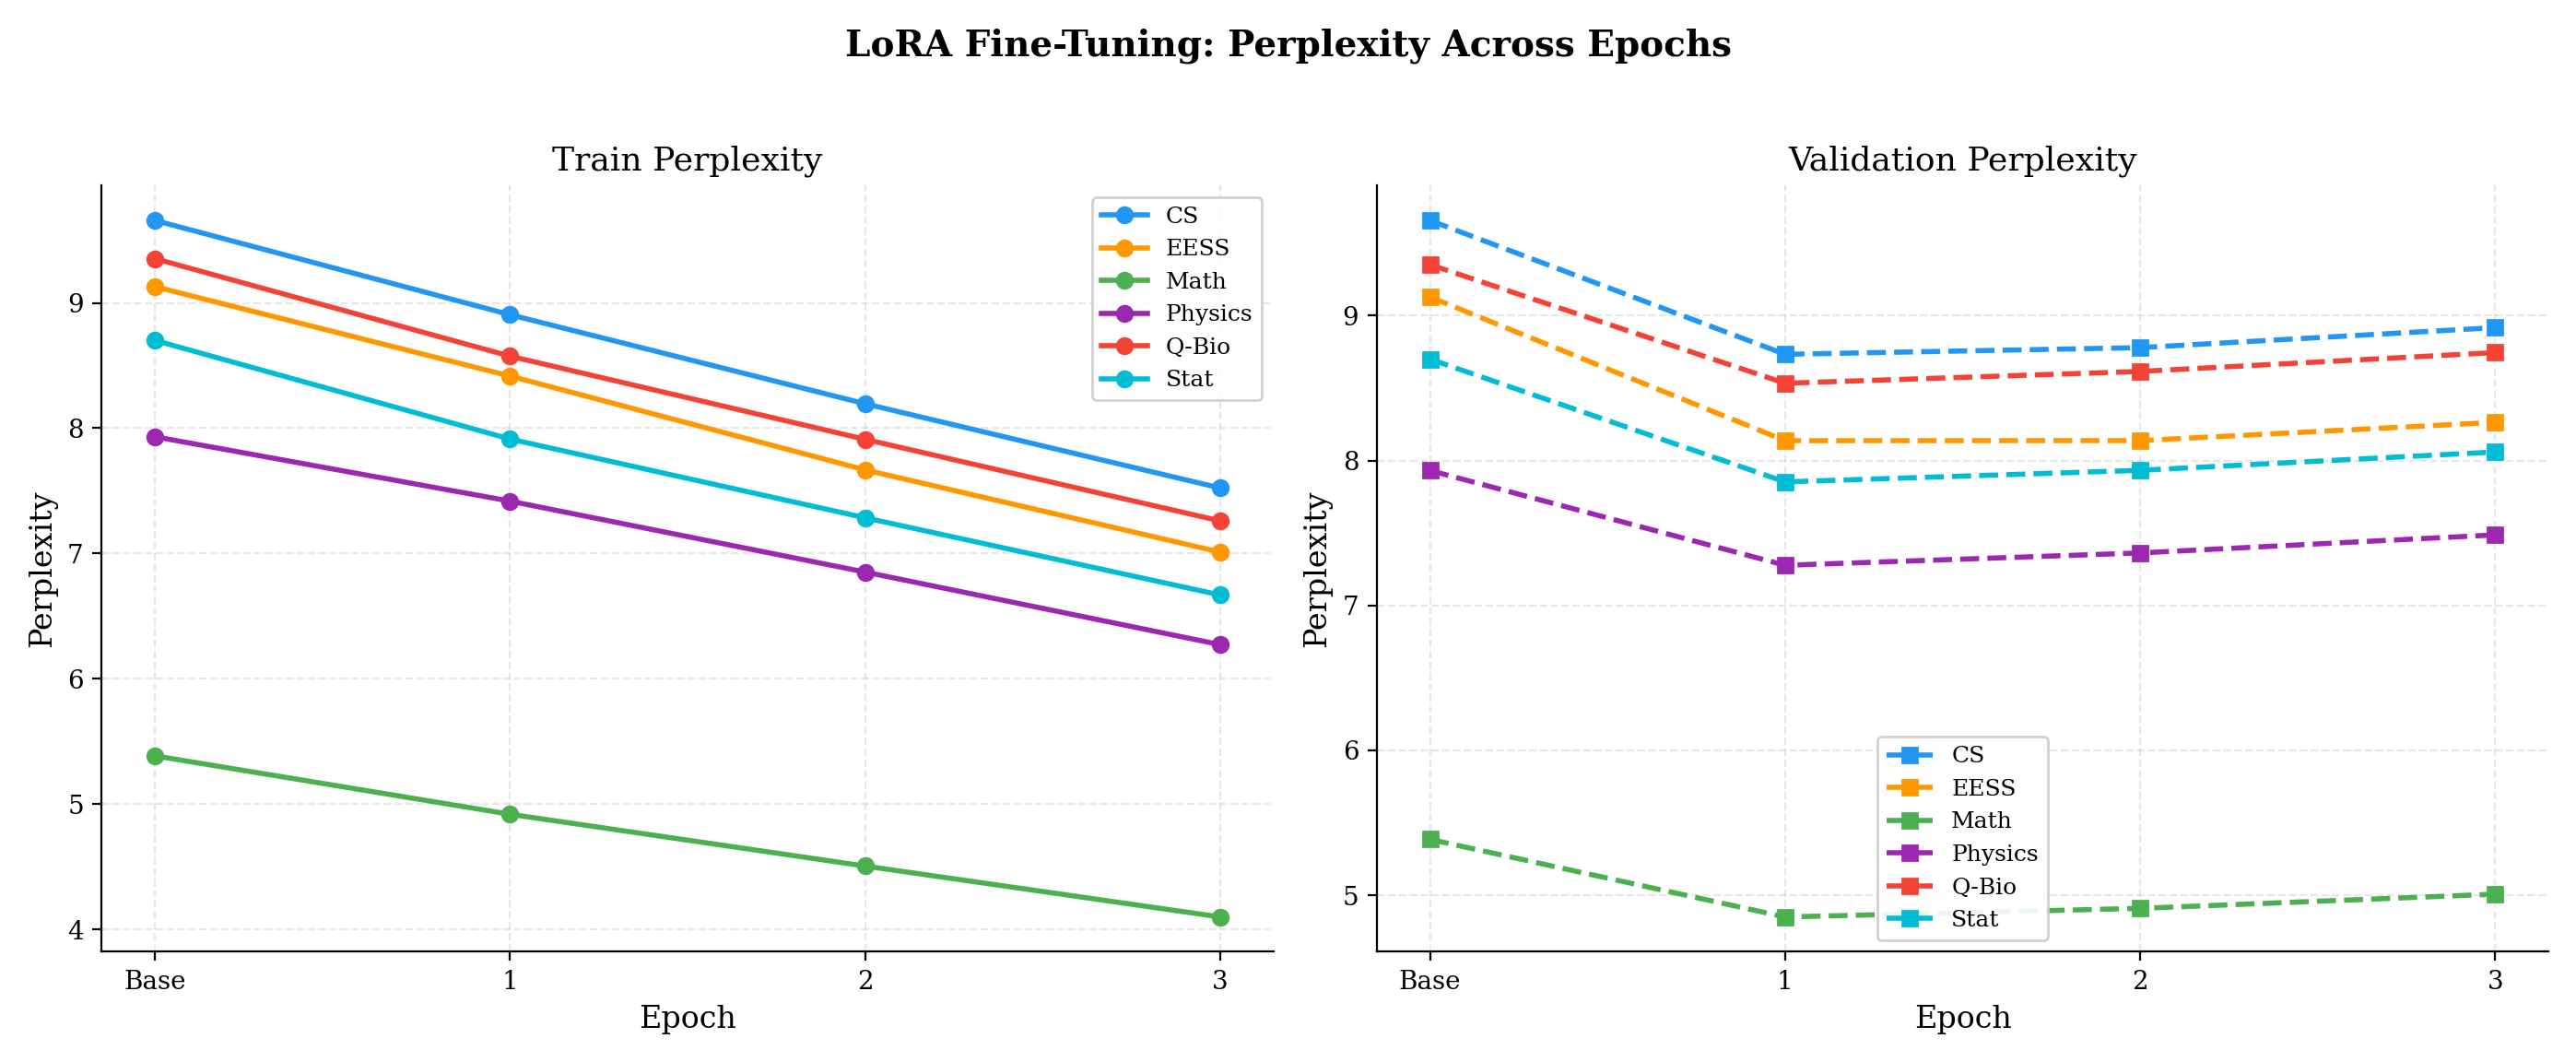
\includegraphics[width=\textwidth]{figures/train_val_perplexity.png}
\caption{Train (left) and validation (right) perplexity across epochs. Epoch 0 denotes the base model baseline. All domains improve on training data; validation diverges after epoch 1.}
\label{fig:perplexity}
\end{figure}

\begin{table}[H]
\centering
\caption{Perplexity across epochs. Best validation in \textbf{bold}.}
\label{tab:perplexity}
\small
\begin{tabular}{l cc cc cc c}
\toprule
& \multicolumn{2}{c}{Epoch 1} & \multicolumn{2}{c}{Epoch 2} & \multicolumn{2}{c}{Epoch 3} & Baseline \\
\cmidrule(lr){2-3} \cmidrule(lr){4-5} \cmidrule(lr){6-7}
Domain & Train & Val & Train & Val & Train & Val & Val \\
\midrule
CS      & 8.91 & \textbf{8.73} & 8.20 & 8.78 & 7.52 & 8.92 & 9.66 \\
EESS    & 8.42 & \textbf{8.14} & 7.67 & 8.14 & 7.01 & 8.26 & 9.13 \\
Math    & 4.92 & \textbf{4.85} & 4.51 & 4.91 & 4.10 & 5.01 & 5.39 \\
Physics & 7.42 & \textbf{7.28} & 6.85 & 7.36 & 6.27 & 7.49 & 7.93 \\
Q-Bio   & 8.57 & \textbf{8.53} & 7.91 & 8.62 & 7.26 & 8.75 & 9.35 \\
Stat    & 7.91 & \textbf{7.85} & 7.29 & 7.93 & 6.67 & 8.06 & 8.70 \\
\bottomrule
\end{tabular}
\end{table}

After exploring multiple configurations, we were unable to prevent overfitting due to the small dataset size (3{,}000 samples per domain). Validation perplexity begins increasing after epoch~1 for all domains while training perplexity continues to decrease. We therefore run all subsequent analyses independently across all three epochs to observe how the attention--MLP adaptation asymmetry evolves as training progresses and the model begins to overfit.


% ======================================================================
\section{Experiment 2.1: Weight Change Norms}
\label{sec:wcn}
% ======================================================================

\subsection{Hypothesis}
MLP weight updates should be \textbf{larger in magnitude} than attention updates, as measured by relative Frobenius norm $\delta = \|\Delta W\|_F / \|W_{\text{base}}\|_F$. This would indicate that MLP modules undergo more substantial adaptation during domain-specific fine-tuning.

\subsection{Method}
For each domain $k$, epoch, layer $\ell$, and module $m$, we compute the effective LoRA update $\Delta W = (\alpha/r) \cdot B A$ and measure:
\[
\delta^{(k),\ell}_m = \frac{\|\Delta W^{(k),\ell}_m\|_F}{\|W^{\ell}_{m,\text{base}}\|_F}
\]
We report both grouped (mean across attention modules vs.\ mean across MLP modules) and per-module breakdowns.

\subsection{Results}

\begin{table}[H]
\centering
\caption{Mean relative weight change norm $\delta$ across all layers (Epoch 3). MLP consistently exceeds attention by 1.24--1.40$\times$.}
\label{tab:wcn}
\small
\begin{tabular}{lccc}
\toprule
Domain & $\bar{\delta}_{\text{attn}}$ & $\bar{\delta}_{\text{mlp}}$ & Ratio \\
\midrule
CS      & 0.00700 & 0.00913 & 1.30$\times$ \\
EESS    & 0.00698 & 0.00976 & 1.40$\times$ \\
Math    & 0.00696 & 0.00864 & 1.24$\times$ \\
Physics & 0.00697 & 0.00870 & 1.25$\times$ \\
Q-Bio   & 0.00705 & 0.00920 & 1.31$\times$ \\
Stat    & 0.00700 & 0.00905 & 1.29$\times$ \\
\bottomrule
\end{tabular}
\end{table}

MLP updates are consistently 1.24--1.40$\times$ larger than attention updates across all domains. The effect is robust: \emph{no domain} violates this pattern. The ratio is modest compared to prior work reporting 2--3$\times$, which is attributable to the difference in base model (Qwen2.5-7B vs.\ Llama) and LoRA targeting all 7 modules rather than a subset.

\begin{figure}[H]
\centering
\begin{subfigure}[b]{0.48\textwidth}
    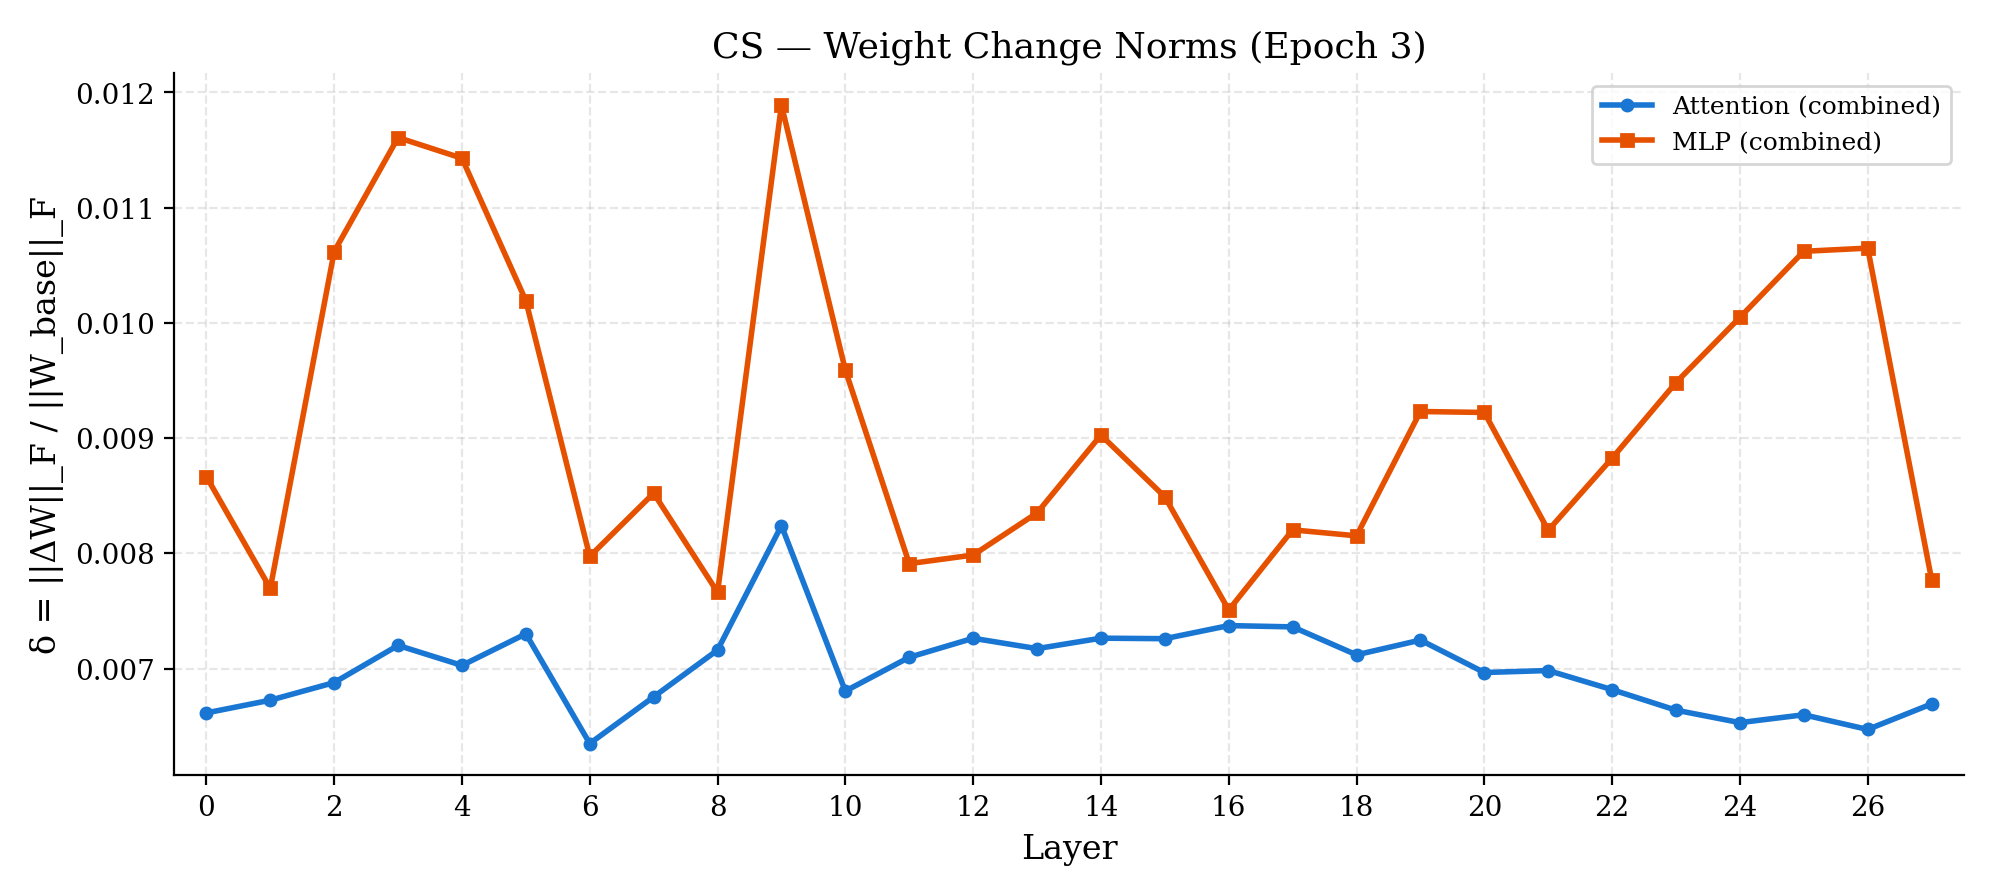
\includegraphics[width=\textwidth]{figures/wcn_cs_grouped.png}
    \caption{CS}
\end{subfigure}
\hfill
\begin{subfigure}[b]{0.48\textwidth}
    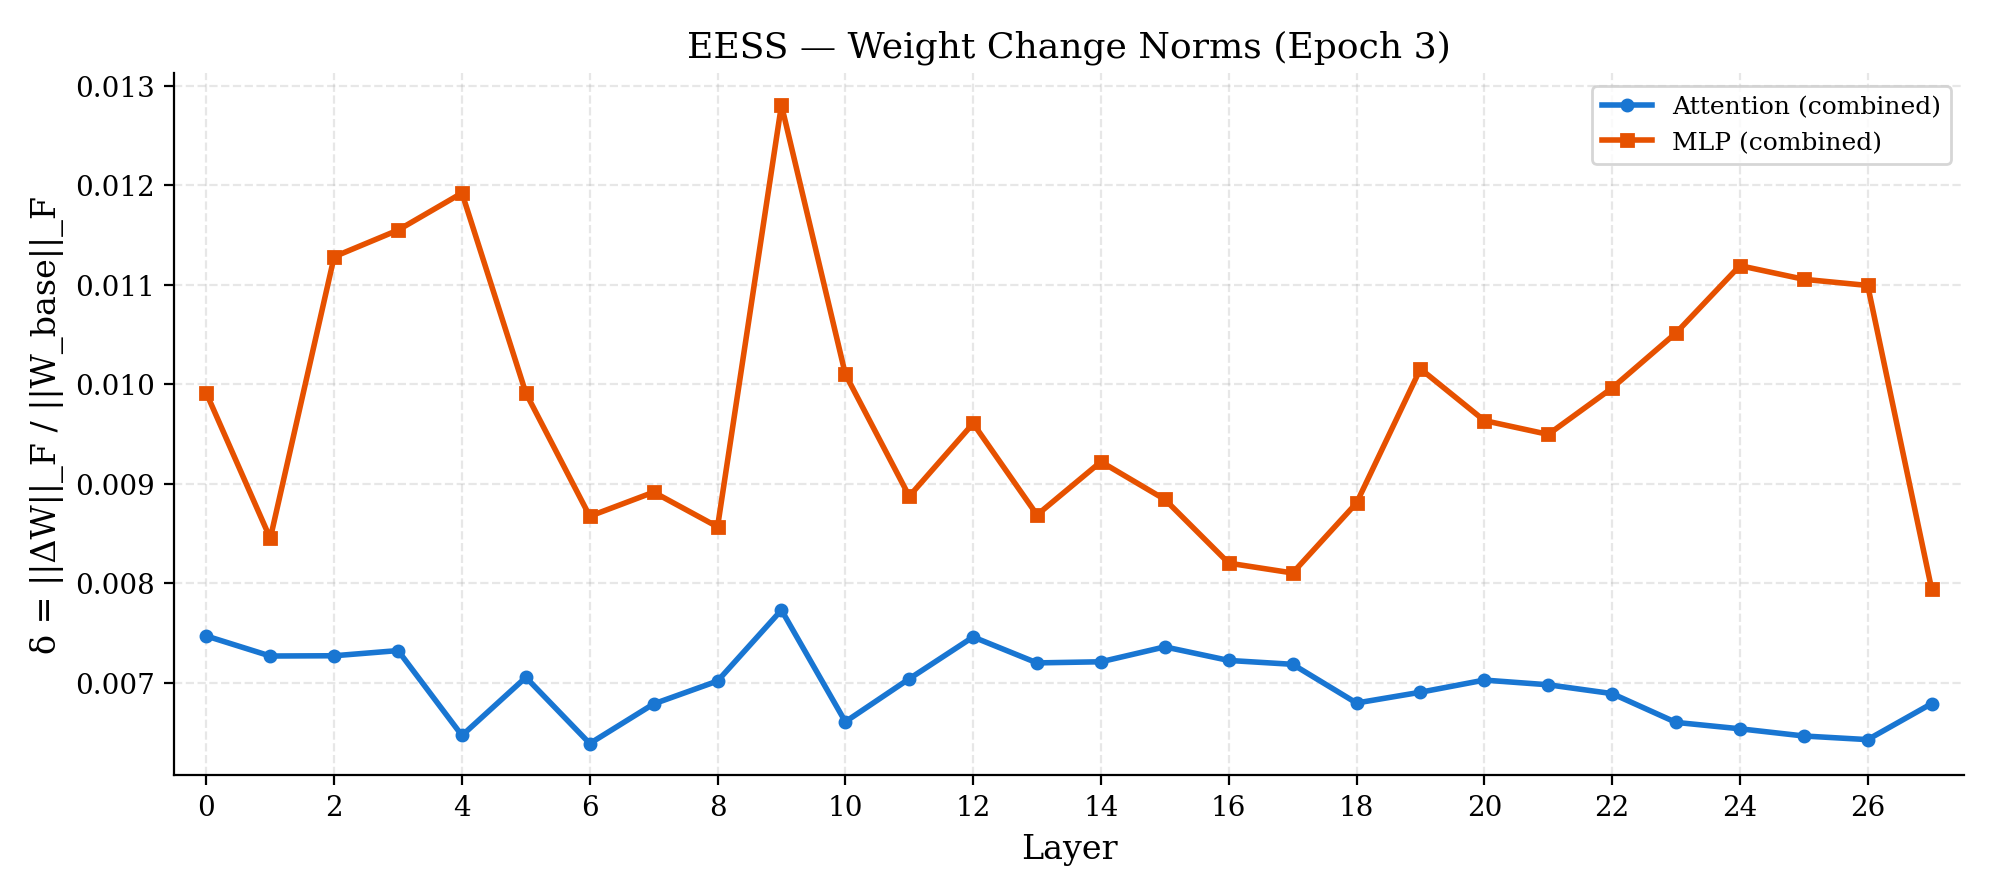
\includegraphics[width=\textwidth]{figures/wcn_eess_grouped.png}
    \caption{EESS}
\end{subfigure}

\vspace{0.3cm}
\begin{subfigure}[b]{0.48\textwidth}
    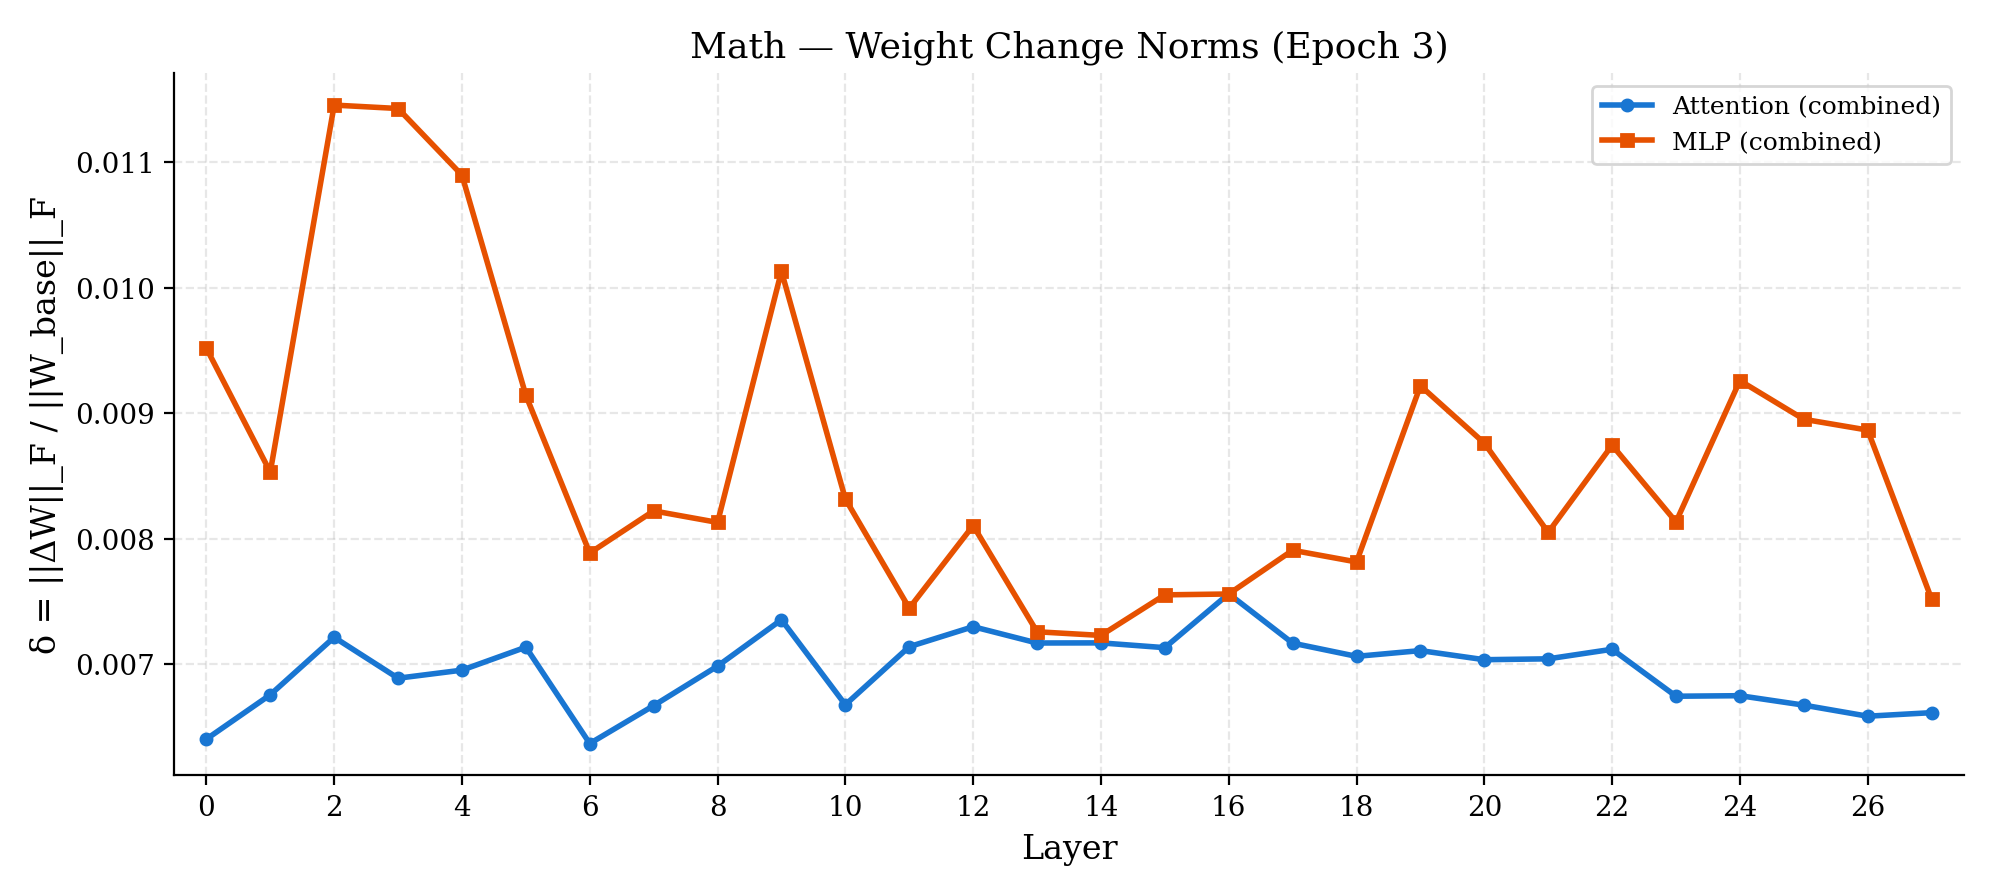
\includegraphics[width=\textwidth]{figures/wcn_math_grouped.png}
    \caption{Math}
\end{subfigure}
\hfill
\begin{subfigure}[b]{0.48\textwidth}
    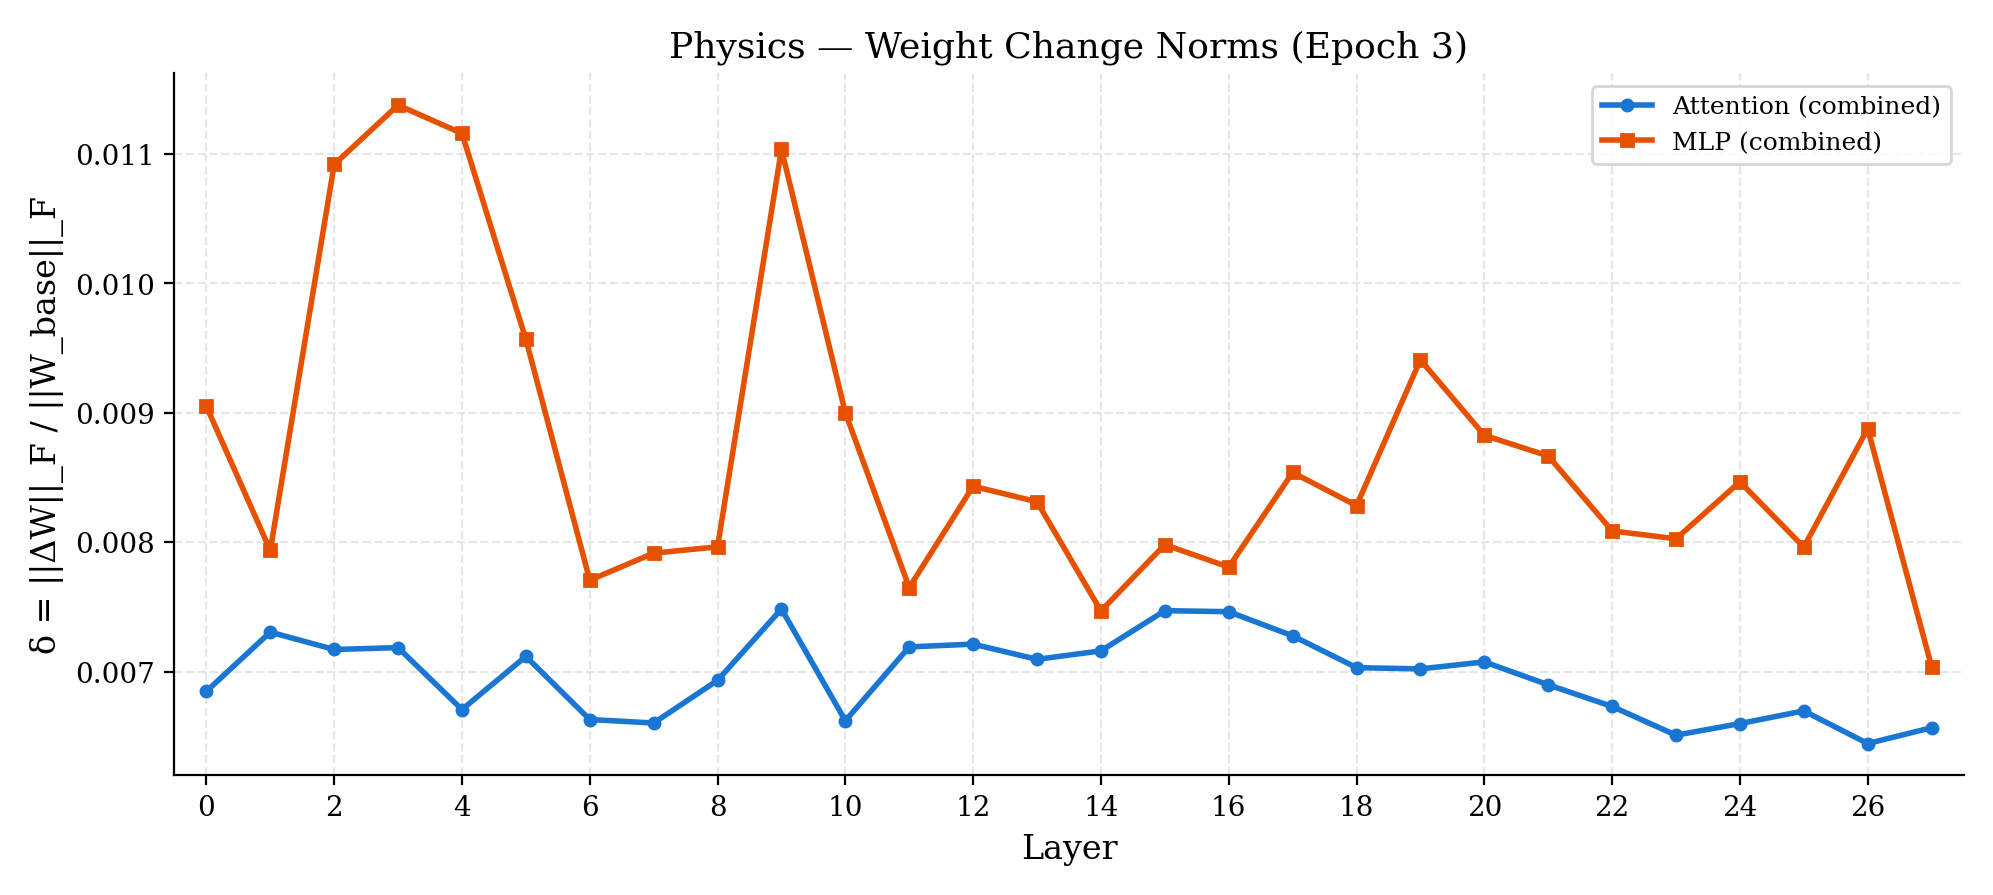
\includegraphics[width=\textwidth]{figures/wcn_physics_grouped.png}
    \caption{Physics}
\end{subfigure}

\vspace{0.3cm}
\begin{subfigure}[b]{0.48\textwidth}
    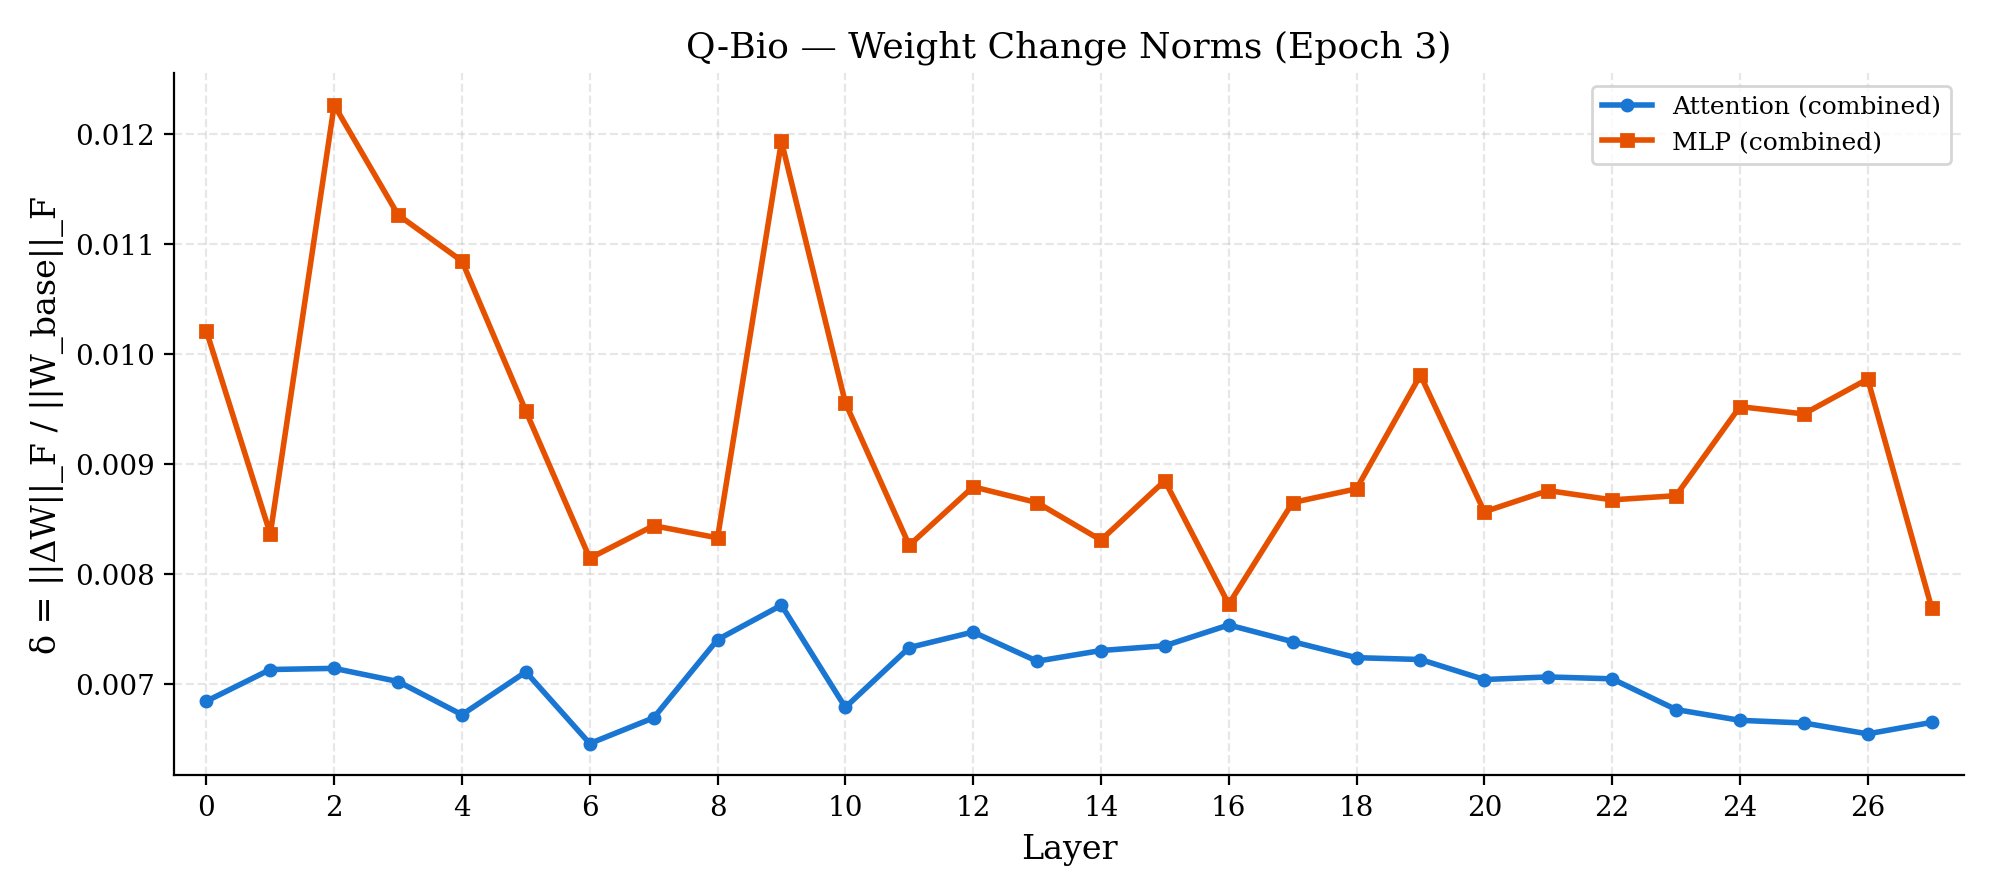
\includegraphics[width=\textwidth]{figures/wcn_q-bio_grouped.png}
    \caption{Q-Bio}
\end{subfigure}
\hfill
\begin{subfigure}[b]{0.48\textwidth}
    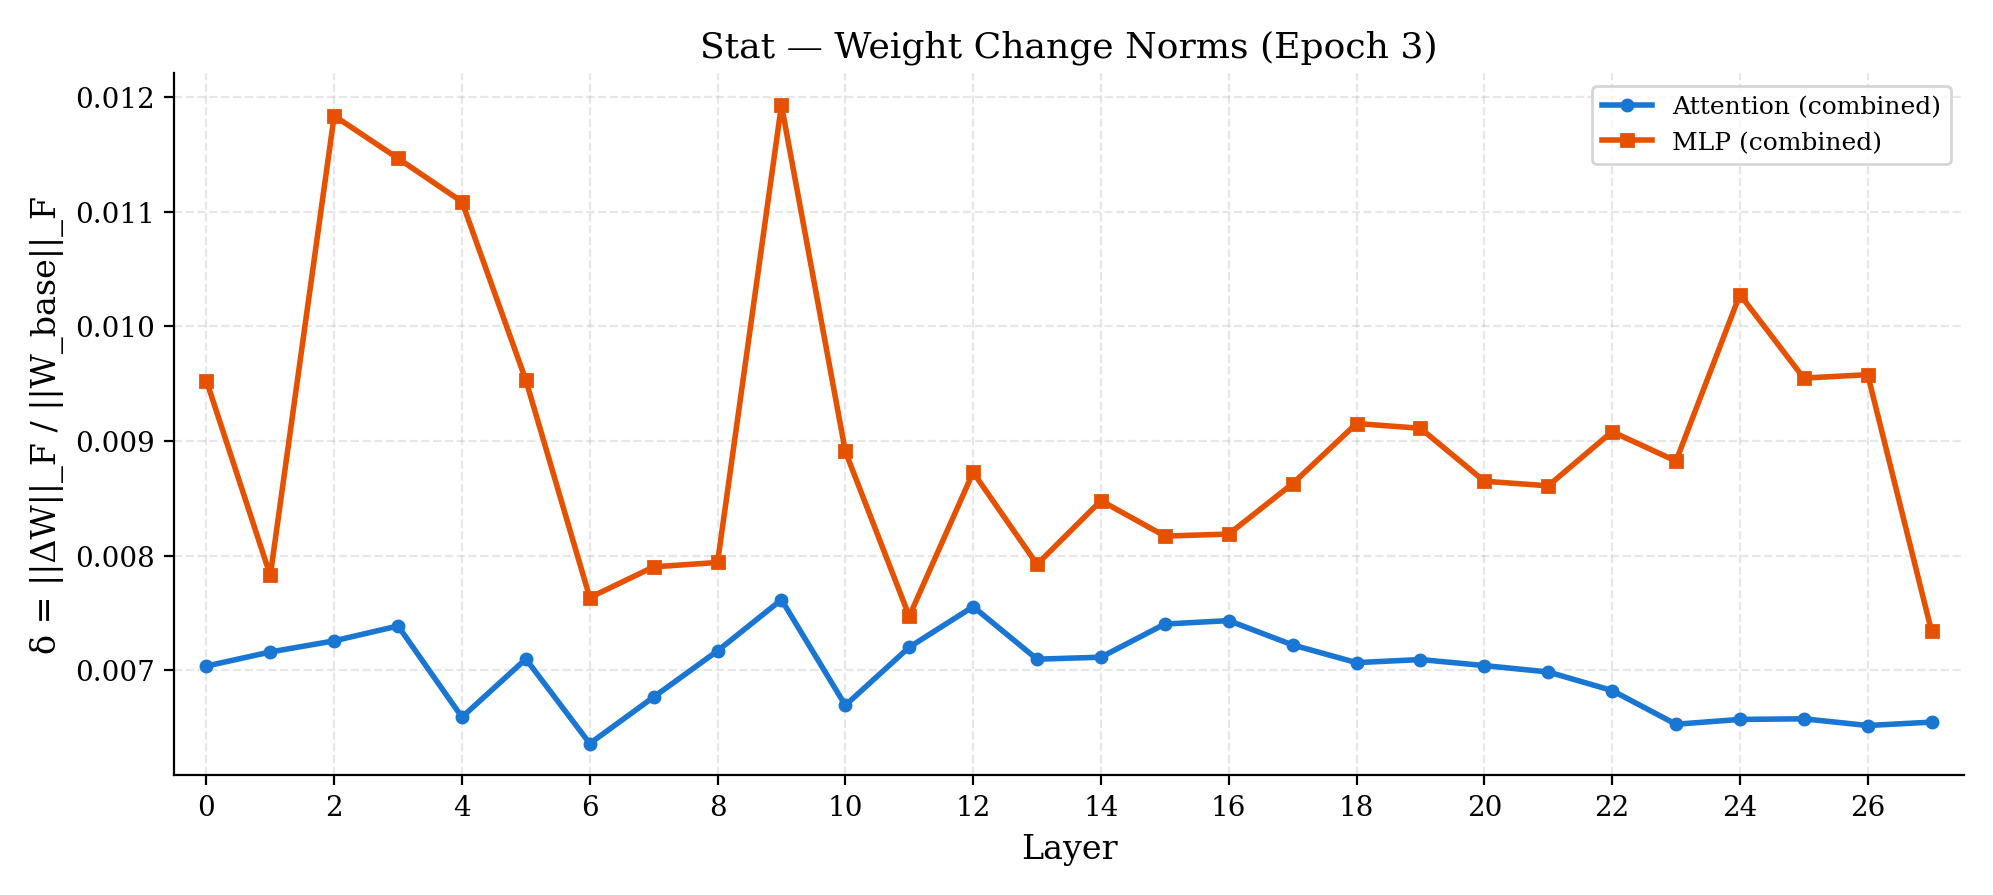
\includegraphics[width=\textwidth]{figures/wcn_stat_grouped.png}
    \caption{Stat}
\end{subfigure}
\caption{Grouped weight change norms ($\delta_{\text{attn}}$ vs.\ $\delta_{\text{mlp}}$) across layers for all six domains (Epoch 3). MLP (orange) consistently exceeds Attention (blue) at nearly every layer.}
\label{fig:wcn_all}
\end{figure}


% ======================================================================
\section{Experiment 2.2: Domain Specificity of Updates}
\label{sec:ds}
% ======================================================================

\subsection{Hypothesis}
MLP weight updates should be more \textbf{domain-differentiated} than attention updates. When fine-tuning on physics, the MLP update should look different from when fine-tuning on math. Attention updates, by contrast, should be more similar across domains --- attention adapts generically regardless of which domain is being learned. This directly addresses the concern that large MLP updates might just reflect a favourable optimisation landscape rather than domain-specific content.

\subsection{Method}
For each layer $\ell$ and module group (attention pooled, MLP pooled), we vectorise the weight updates from all six domains and compute pairwise cosine similarity:
\[
\text{sim}(k, k')^{\ell} = \frac{\langle \text{vec}(\Delta W_\ell^{(k)}),\; \text{vec}(\Delta W_\ell^{(k')}) \rangle}{\|\text{vec}(\Delta W_\ell^{(k)})\| \cdot \|\text{vec}(\Delta W_\ell^{(k')})\|}
\]

This produces a $6 \times 6$ cross-domain similarity matrix at each layer. We summarise this with two \textbf{domain mixing} scalar metrics, computed over off-diagonal elements:
\begin{itemize}
    \item \textbf{MSE mixing score}: $\text{mean}(S_{\text{offdiag}}^2)$ --- penalises large cross-domain similarity quadratically.
    \item \textbf{MAE mixing score}: $\text{mean}(|S_{\text{offdiag}}|)$ --- linear average of cross-domain similarity.
\end{itemize}
Both range from 0 (perfectly domain-specialised, identity-like matrix) to 1 (fully domain-mixed, uniform matrix).

\subsection{Results}

The prediction is confirmed: MLP updates are consistently more domain-differentiated (lower mixing scores) than attention updates.

\begin{table}[H]
\centering
\caption{Domain mixing scores --- grand mean across all 28 layers (Epoch 3). Lower = more domain-specialised.}
\label{tab:mixing}
\begin{tabular}{lcc}
\toprule
Metric & Attention & MLP \\
\midrule
MSE ($\text{mean}(S^2_{\text{offdiag}})$) & 0.0275 & 0.0118 \\
MAE ($\text{mean}(|S_{\text{offdiag}}|)$)  & 0.1387 & 0.0880 \\
Mean off-diagonal similarity                & 0.1387 & 0.0880 \\
\bottomrule
\end{tabular}
\end{table}

By the MSE metric, MLP is $2.3\times$ more domain-specialised than attention. By MAE, the ratio is $1.6\times$. The MSE metric amplifies the signal because attention has a few high cross-domain pairs (e.g.\ v\_proj) that are penalised quadratically.

\begin{figure}[H]
\centering
\begin{subfigure}[b]{0.48\textwidth}
    
\includegraphics[width=\textwidth]{figures/domain_mixing_layerwise_mse.png}
    \caption{MSE mixing score across layers.}
\end{subfigure}
\hfill
\begin{subfigure}[b]{0.48\textwidth}
    
\includegraphics[width=\textwidth]{figures/domain_mixing_layerwise_mae.png}
    \caption{MAE mixing score across layers.}
\end{subfigure}
\caption{Domain mixing scores across layers (Epoch 3). Higher values indicate more domain-mixed (less specialised) updates. Attention (blue) consistently shows higher mixing than MLP (orange), especially in early layers (0--9).}
\label{fig:mixing_layerwise}
\end{figure}

\begin{figure}[H]
\centering

\includegraphics[width=\textwidth]{figures/domain_mixing_summary.png}
\caption{Per-module domain mixing summary (grand mean across all layers, Epoch 3). Blue = attention modules, orange = MLP modules. \texttt{gate\_proj} is the most domain-specialised module overall (lowest mixing score). Among attention modules, \texttt{v\_proj} is the most domain-mixed.}
\label{fig:mixing_summary}
\end{figure}

\paragraph{Module-wise drill-down.} To identify which specific modules drive the attention--MLP gap, we examine the single most distinguishing layer --- the layer where the off-diagonal similarity gap between attention and MLP is largest. For Epoch 3, this is \textbf{Layer 5} (attention off-diag mean = 0.266, MLP off-diag mean = 0.125, gap = 0.141).

\begin{figure}[H]
\centering

\includegraphics[width=\textwidth]{figures/modulewise_most_distinguishing_layer.png}
\caption{Module-wise $6 \times 6$ similarity heatmaps at Layer 5 (Epoch 3). Top row: attention modules (q/k/v\_proj). Middle: o\_proj and pooled groups. Bottom: MLP modules (gate/up/down\_proj). All share a common colour scale. \texttt{gate\_proj} (bottom-left) shows near-zero off-diagonal similarity --- almost perfectly domain-specialised. \texttt{v\_proj} (top-right) shows the highest cross-domain similarity within attention.}
\label{fig:modulewise}
\end{figure}


% ======================================================================
\section{Experiment 2.3: Domain Alignment}
\label{sec:alignment}
% ======================================================================

\subsection{Hypothesis}
MLP weight updates should be more \textbf{aligned with domain concept vectors} than attention updates. The domain concept vectors $\hat{d}^{\ell}_k$ (computed from the forward pass geometry in Experiment 1) define the directions in representation space that carry domain identity. If MLP stores domain-specific knowledge, its weight updates should specifically modify these directions, rather than changing weights in orthogonal, domain-irrelevant directions.

\subsection{Method}
We measure domain alignment using two complementary metrics:

\paragraph{Projection metric ($\rho$).} For each domain $k$, layer $\ell$, and module $m$:
\[
\rho^{(k),\ell}_m = \frac{\|\Delta W^{(k),\ell}_m \cdot \hat{d}^{\text{mlp},\ell}_k\|}{\|\Delta W^{(k),\ell}_m\|_F}
\]
This measures: when the weight update is applied to the domain concept direction, how large is the output relative to the total update norm? High $\rho$ means the update specifically operates on the domain-identity direction.

We pool across modules within each group (attention vs.\ MLP) using Frobenius-norm weighting: $\rho_{\text{pooled}} = \sum_m w_m \rho_m / \sum_m w_m$, where $w_m = \|\Delta W_m\|_F$.

\paragraph{SVD overlap metric.} Compute the SVD of $\Delta W$ and measure the total squared overlap of its top singular vectors with $\hat{d}^{\ell}_k$. This captures whether the principal directions of the weight update contain the domain concept direction, independent of magnitude.

\subsection{Results}

MLP updates show $2\text{--}4\times$ higher alignment with domain concept vectors than attention updates, consistently across all six domains.

\begin{table}[H]
\centering
\caption{Mean domain alignment $\rho$ across all layers (Epoch 3, mean pool). MLP exceeds attention by $2\text{--}4\times$ for every domain.}
\label{tab:alignment}
\small
\begin{tabular}{lccc}
\toprule
Domain & $\bar{\rho}_{\text{attn}}$ & $\bar{\rho}_{\text{mlp}}$ & Ratio \\
\midrule
CS      & 0.0205 & 0.0678 & 3.31$\times$ \\
EESS    & 0.0205 & 0.0802 & 3.92$\times$ \\
Math    & 0.0174 & 0.0359 & 2.06$\times$ \\
Physics & 0.0175 & 0.0554 & 3.16$\times$ \\
Q-Bio   & 0.0177 & 0.0411 & 2.32$\times$ \\
Stat    & 0.0188 & 0.0549 & 2.92$\times$ \\
\bottomrule
\end{tabular}
\end{table}

\begin{figure}[H]
\centering
\begin{subfigure}[b]{0.48\textwidth}
    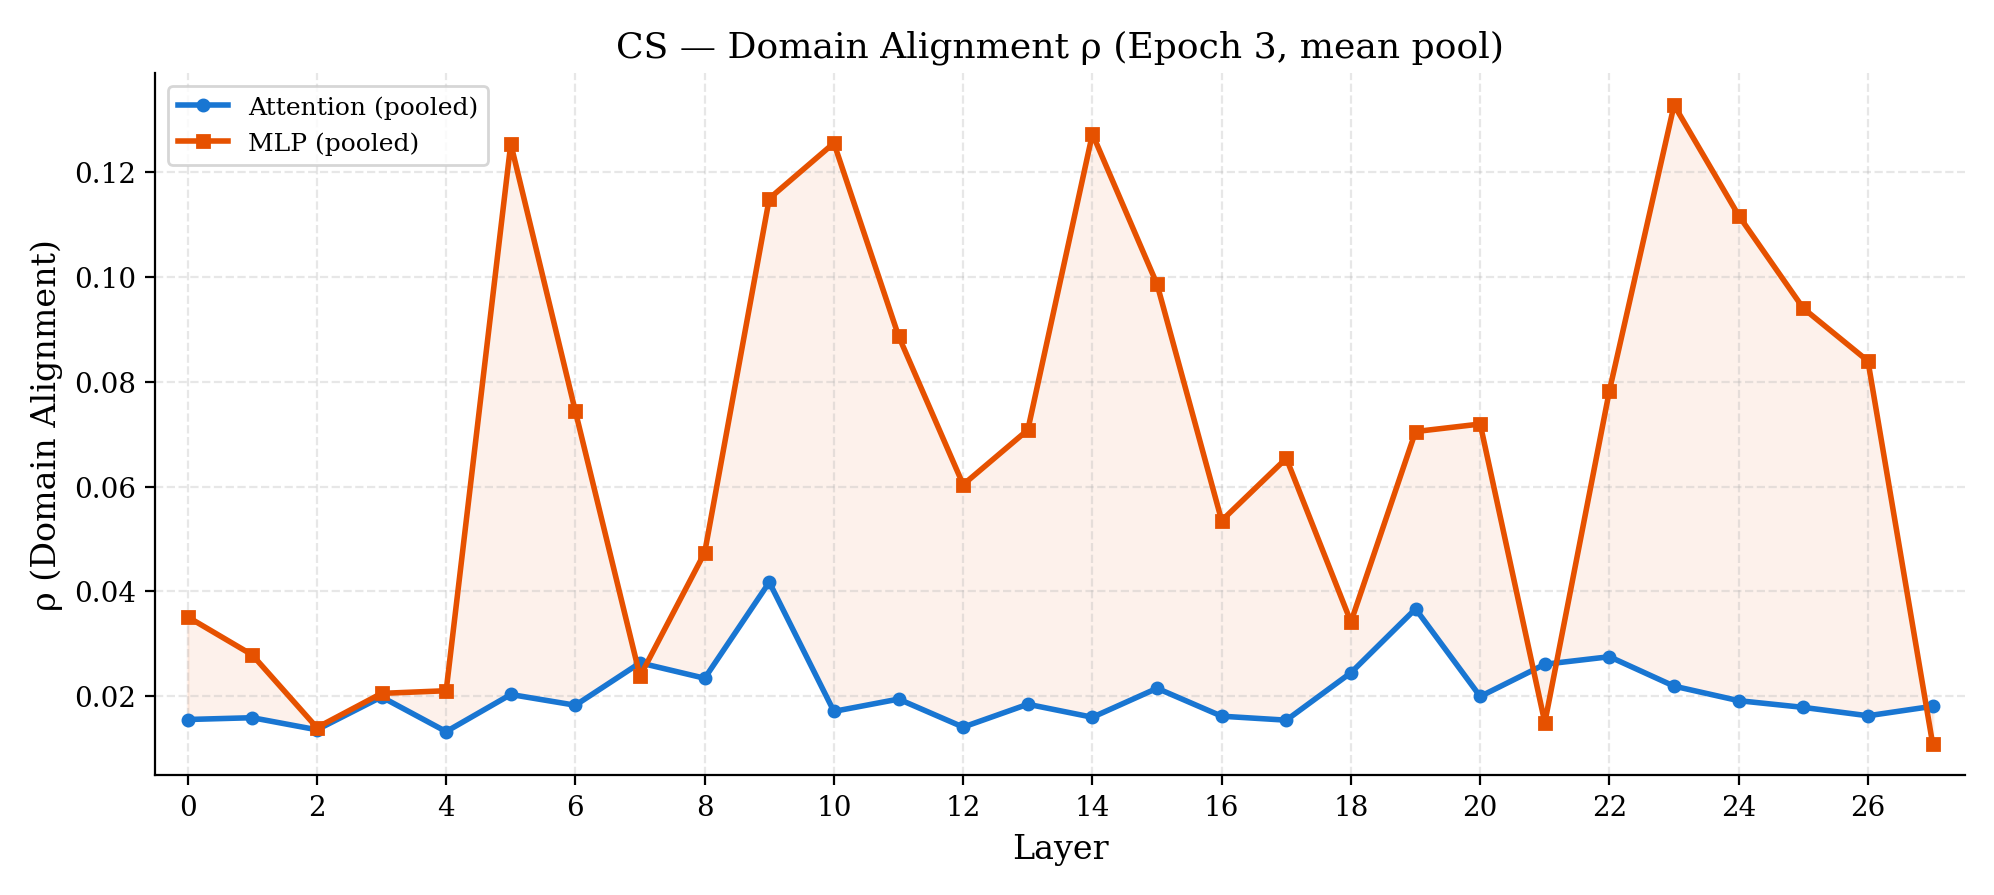
\includegraphics[width=\textwidth]{figures/proj_cs.png}
    \caption{Projection $\rho$: CS}
\end{subfigure}
\hfill
\begin{subfigure}[b]{0.48\textwidth}
    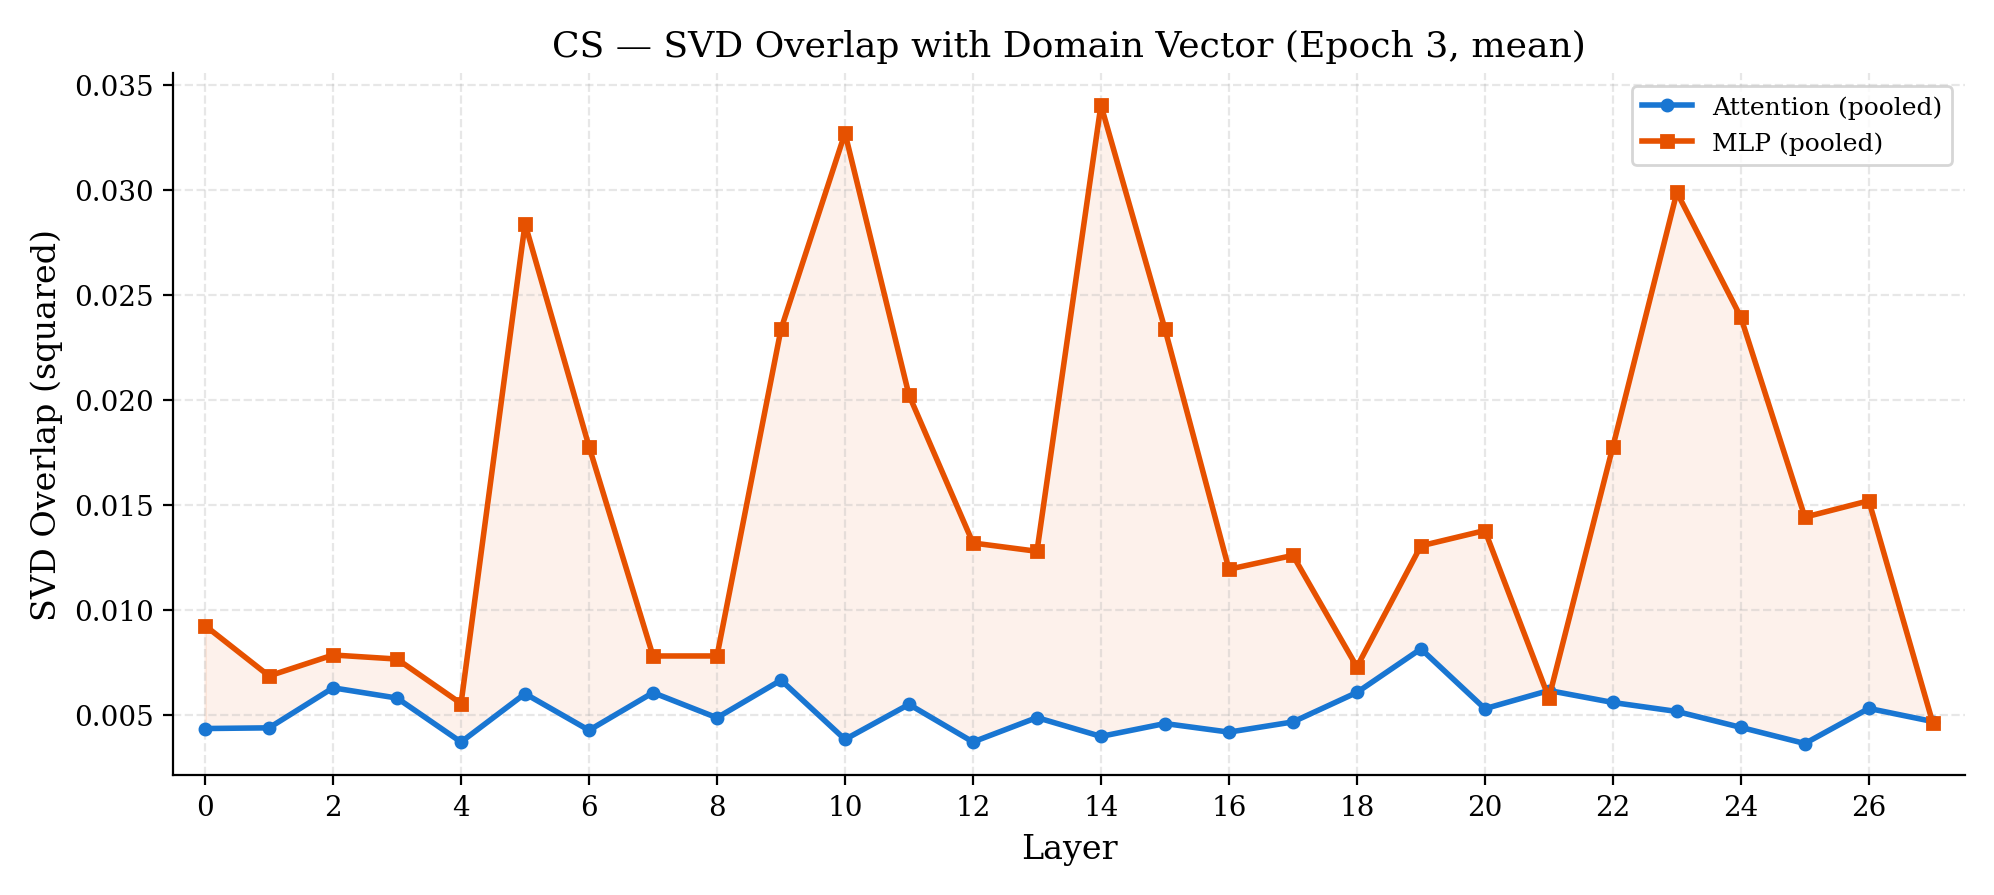
\includegraphics[width=\textwidth]{figures/svd_cs.png}
    \caption{SVD overlap: CS}
\end{subfigure}
\caption{Domain alignment across layers for CS (Epoch 3, mean pool). Left: projection metric $\rho$. Right: SVD overlap. In both, MLP (orange) dramatically exceeds attention (blue), with sharp peaks at layers 5, 10, 14, and 23.}
\label{fig:alignment_cs}
\end{figure}

\begin{figure}[H]
\centering
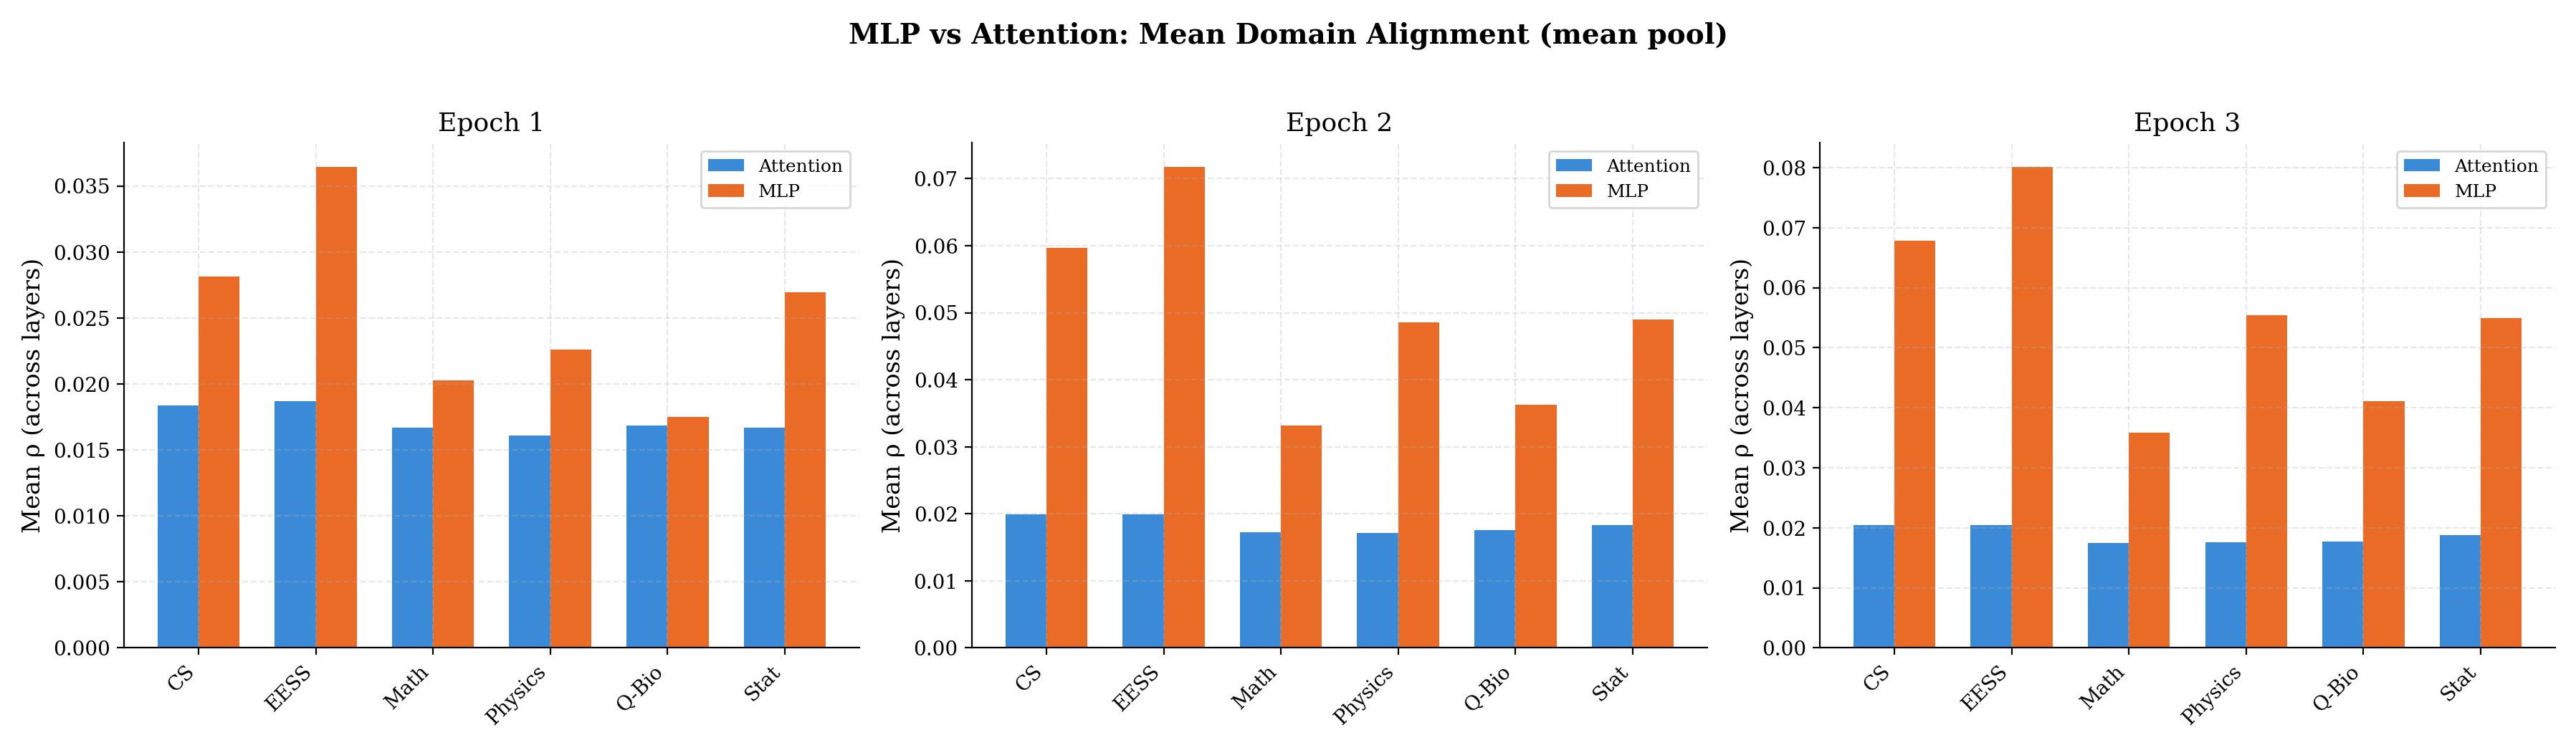
\includegraphics[width=\textwidth]{figures/alignment_summary_bar.png}
\caption{Summary: mean $\rho$ across layers for all domains and all three epochs (mean pool). MLP consistently exceeds attention, and the gap \emph{widens} with more training.}
\label{fig:alignment_summary}
\end{figure}

The alignment gap grows across epochs: at Epoch 1, the MLP/Attention ratio is ${\sim}1.5\text{--}2\times$; by Epoch 3, it reaches $2\text{--}4\times$. This indicates that as the model trains longer, MLP updates become increasingly targeted toward domain-specific directions --- even as the model begins to overfit on validation loss. The domain concept vectors act as a \emph{directional signature} that MLP adapts toward.


% ======================================================================
\section{Special Finding: The \texttt{gate\_proj} Anomaly}
\label{sec:gate}
% ======================================================================

Across all three experiments, the \texttt{gate\_proj} matrix shows anomalously strong domain-specific behaviour, standing out from all other modules.

\subsection{What is \texttt{gate\_proj}?}

In the SwiGLU MLP architecture used by Qwen2.5 (and Llama-family models), the MLP block at each layer computes:
\[
\text{MLP}(x) = W_{\text{down}} \cdot \bigl[\sigma(W_{\text{gate}} \cdot x) \odot (W_{\text{up}} \cdot x)\bigr]
\]
where $\sigma$ is the SiLU activation and $\odot$ is element-wise multiplication. The \texttt{gate\_proj} ($W_{\text{gate}}$) acts as a \textbf{feature amplifier}: it controls which intermediate features are activated via the gating mechanism. By selectively amplifying or suppressing features, it determines what information passes through the MLP. This makes it a natural locus for domain-specific adaptation.

\subsection{Evidence Across Experiments}

\begin{table}[H]
\centering
\caption{\texttt{gate\_proj} vs.\ other modules (averaged across all domains, Epoch 3).}
\label{tab:gate}
\begin{tabular}{lccc}
\toprule
Module & $\bar{\delta}$ (weight norm) & $\bar{\rho}$ (alignment) & MSE mixing \\
\midrule
q\_proj     & 0.00685 & 0.0215 & 0.0107 \\
k\_proj     & 0.00658 & 0.0171 & 0.0145 \\
v\_proj     & 0.00765 & 0.0197 & 0.0902 \\
o\_proj     & 0.00744 & 0.0162 & 0.0431 \\
\midrule
\textbf{gate\_proj} & \textbf{0.01230} & \textbf{0.0767} & \textbf{0.0036} \\
up\_proj    & 0.00816 & 0.0338 & 0.0224 \\
down\_proj  & 0.00466 & 0.0297 & 0.0499 \\
\bottomrule
\end{tabular}
\end{table}

\begin{itemize}
    \item \textbf{Weight change norm}: \texttt{gate\_proj} has the highest $\delta$ of any module ($0.0123$), nearly $1.8\times$ the next-highest (up\_proj at $0.0082$) and $1.7\times$ the attention average.
    \item \textbf{Domain alignment}: \texttt{gate\_proj} has the highest $\rho$ ($0.0767$), more than $2\times$ the next-highest MLP module (up\_proj at $0.0338$) and $3.8\times$ the attention average.
    \item \textbf{Domain specificity}: \texttt{gate\_proj} has the \emph{lowest} MSE mixing score ($0.0036$), meaning its updates are the most domain-differentiated of any module. It is $6\times$ more specialised than up\_proj.
\end{itemize}

\begin{figure}[H]
\centering
\begin{subfigure}[b]{0.48\textwidth}
    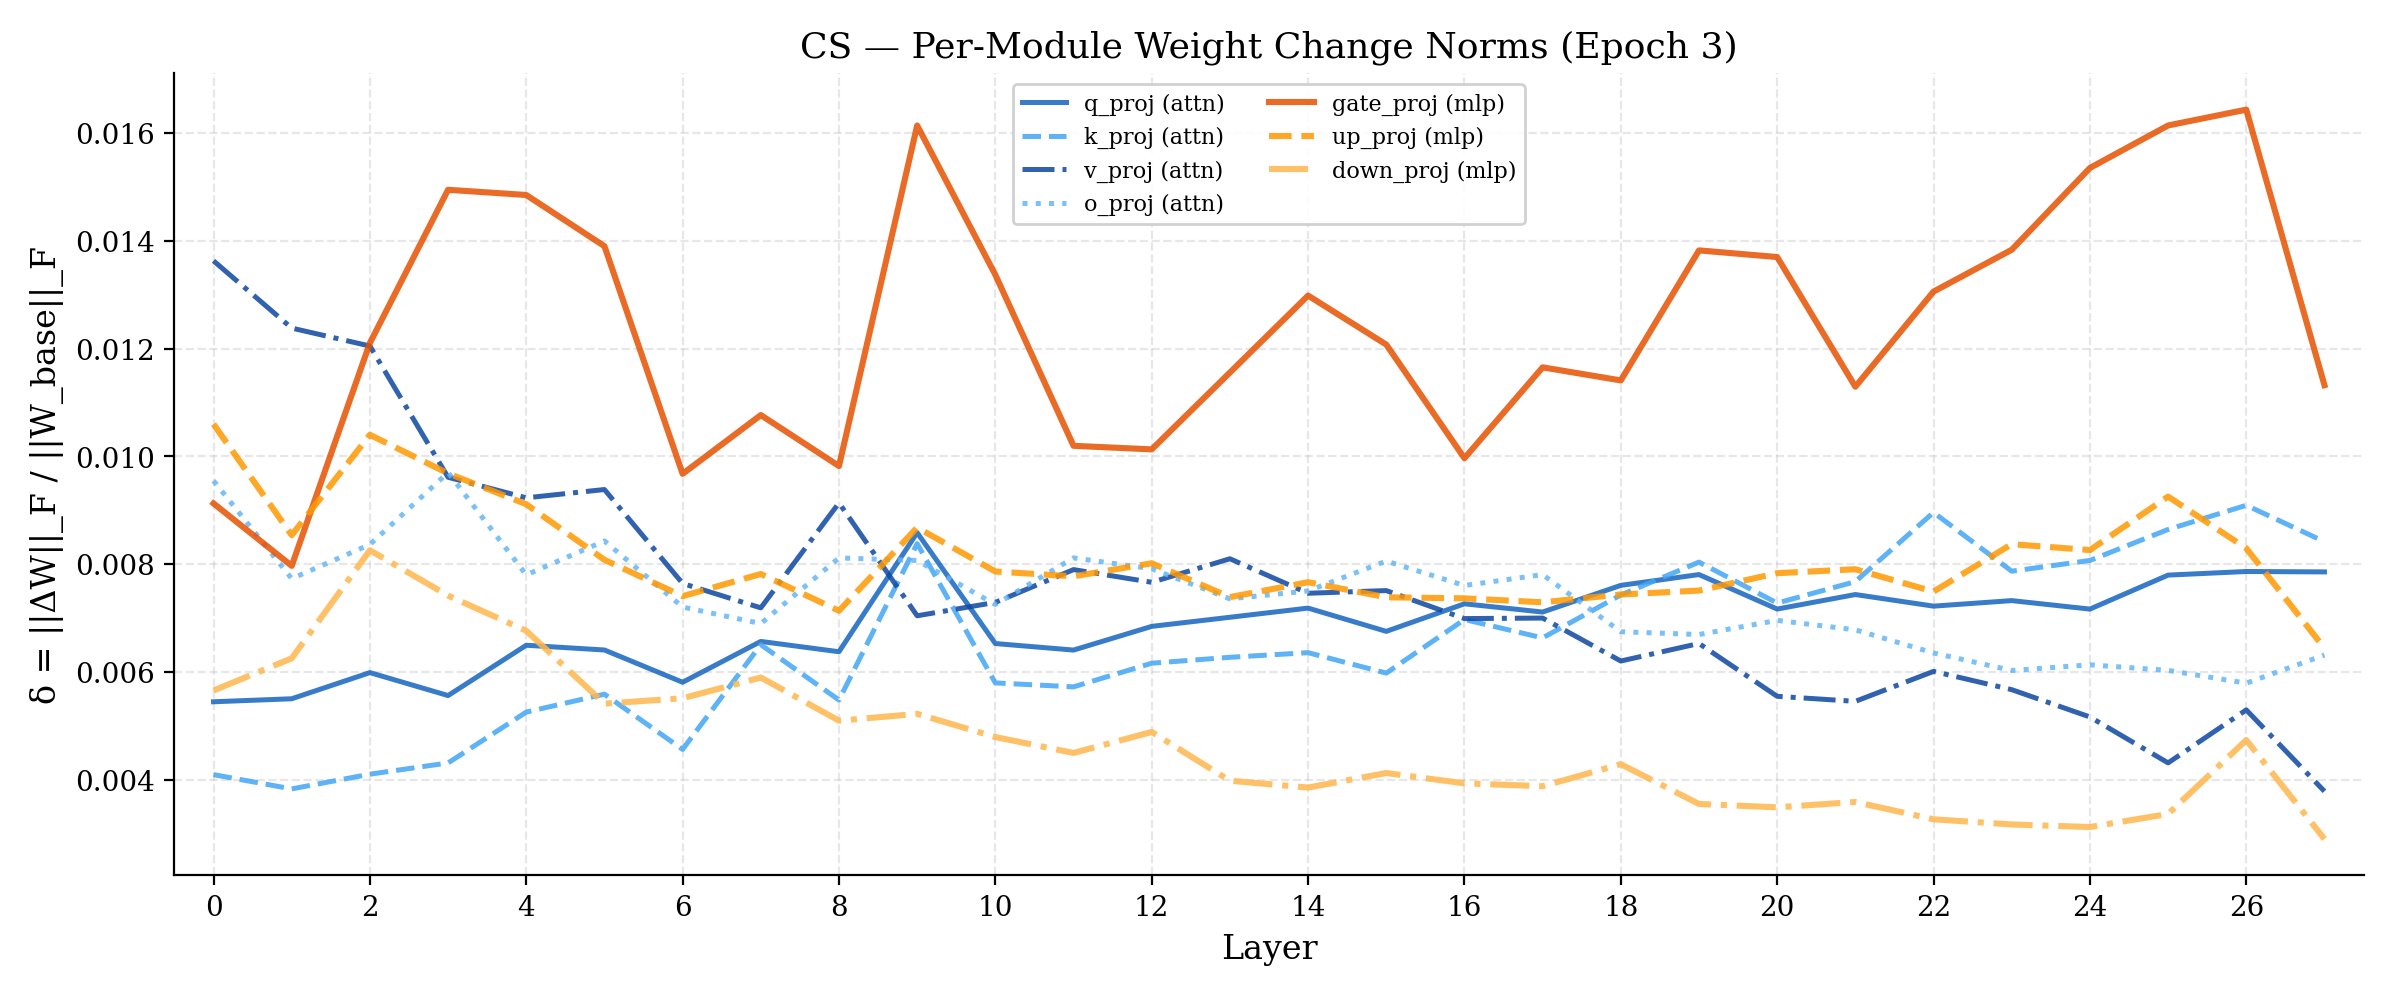
\includegraphics[width=\textwidth]{figures/wcn_cs_detailed.png}
    \caption{Per-module weight change norms (CS).}
\end{subfigure}
\hfill
\begin{subfigure}[b]{0.48\textwidth}
    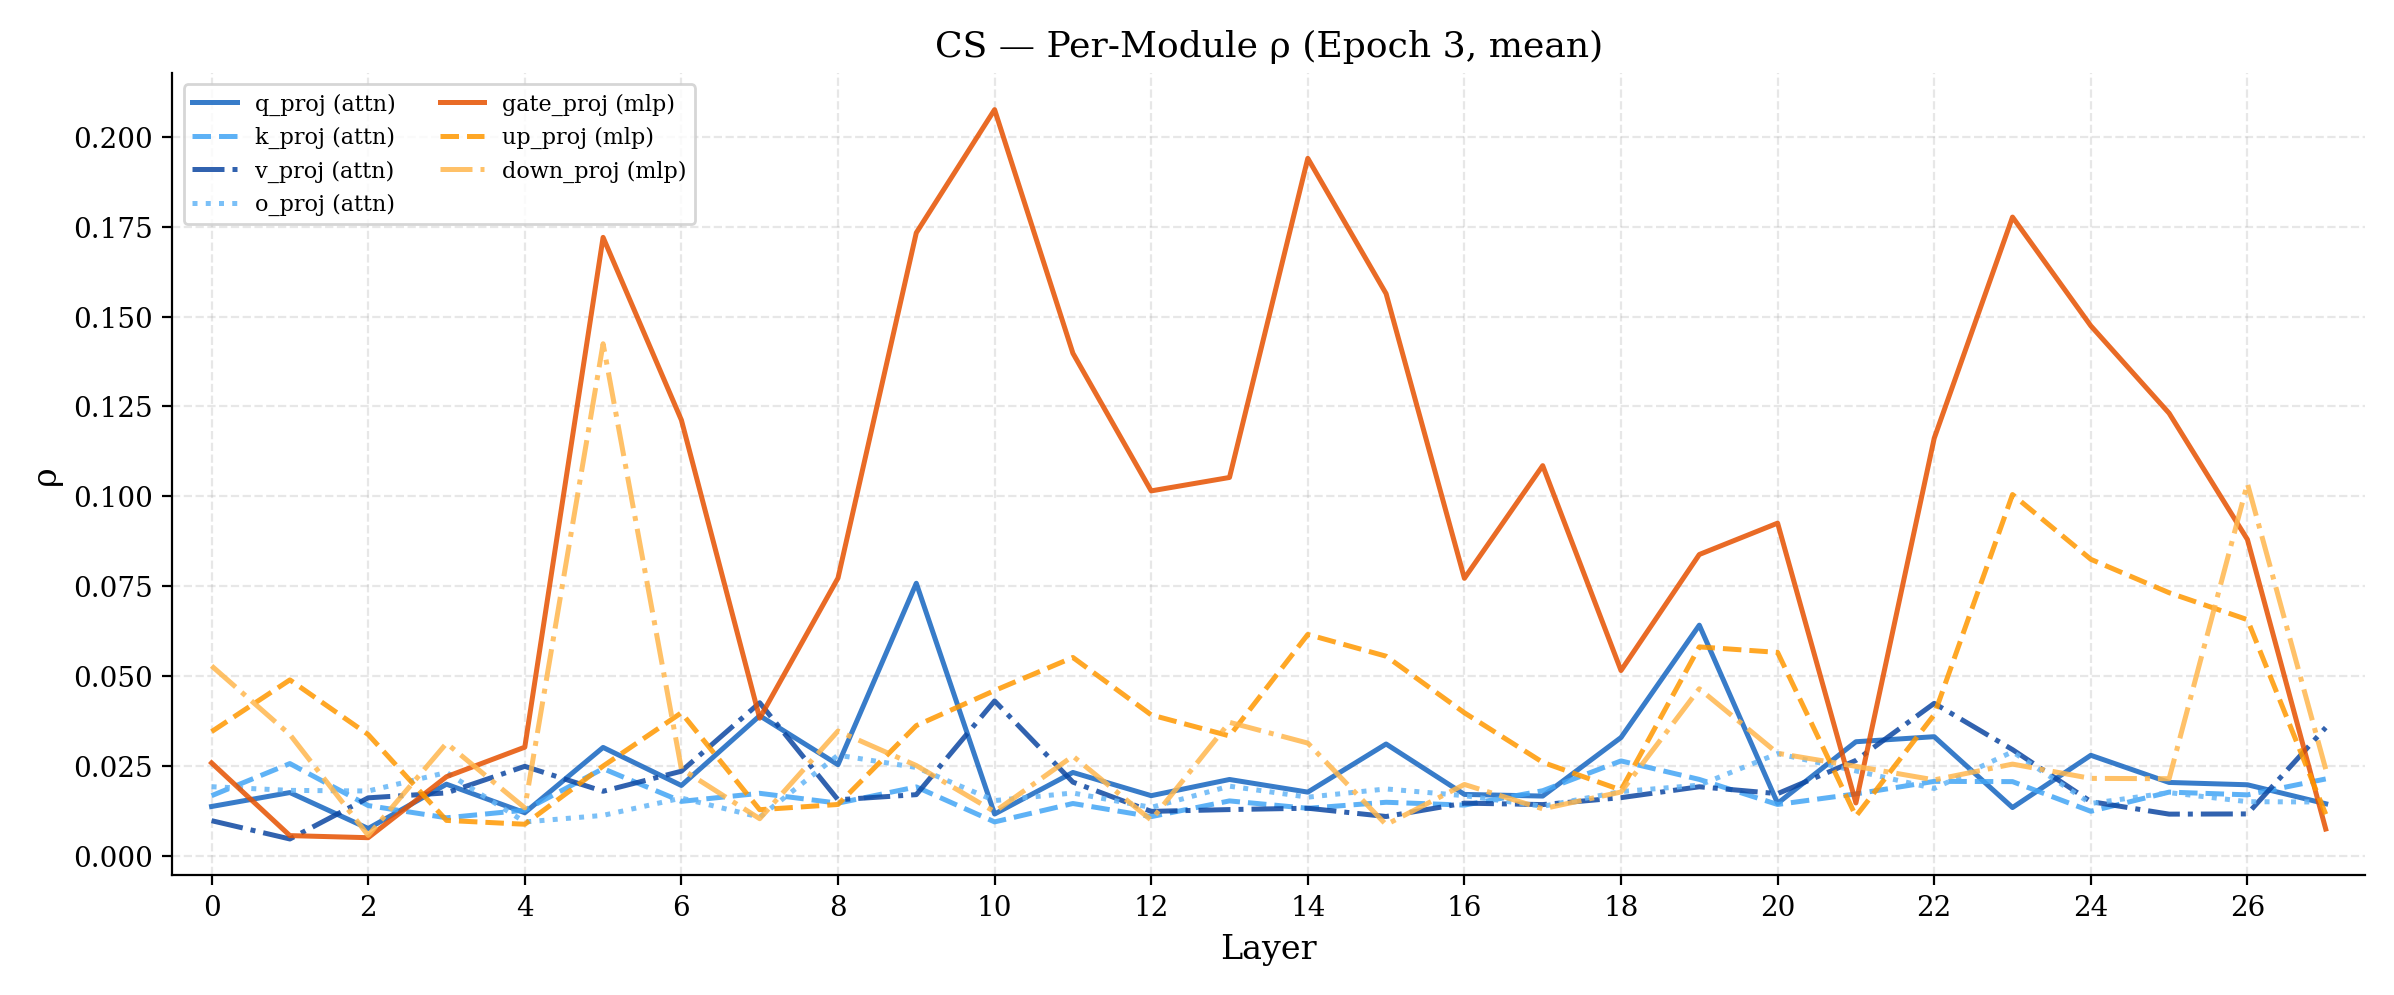
\includegraphics[width=\textwidth]{figures/permod_cs.png}
    \caption{Per-module domain alignment $\rho$ (CS).}
\end{subfigure}

\vspace{0.3cm}
\begin{subfigure}[b]{0.48\textwidth}
    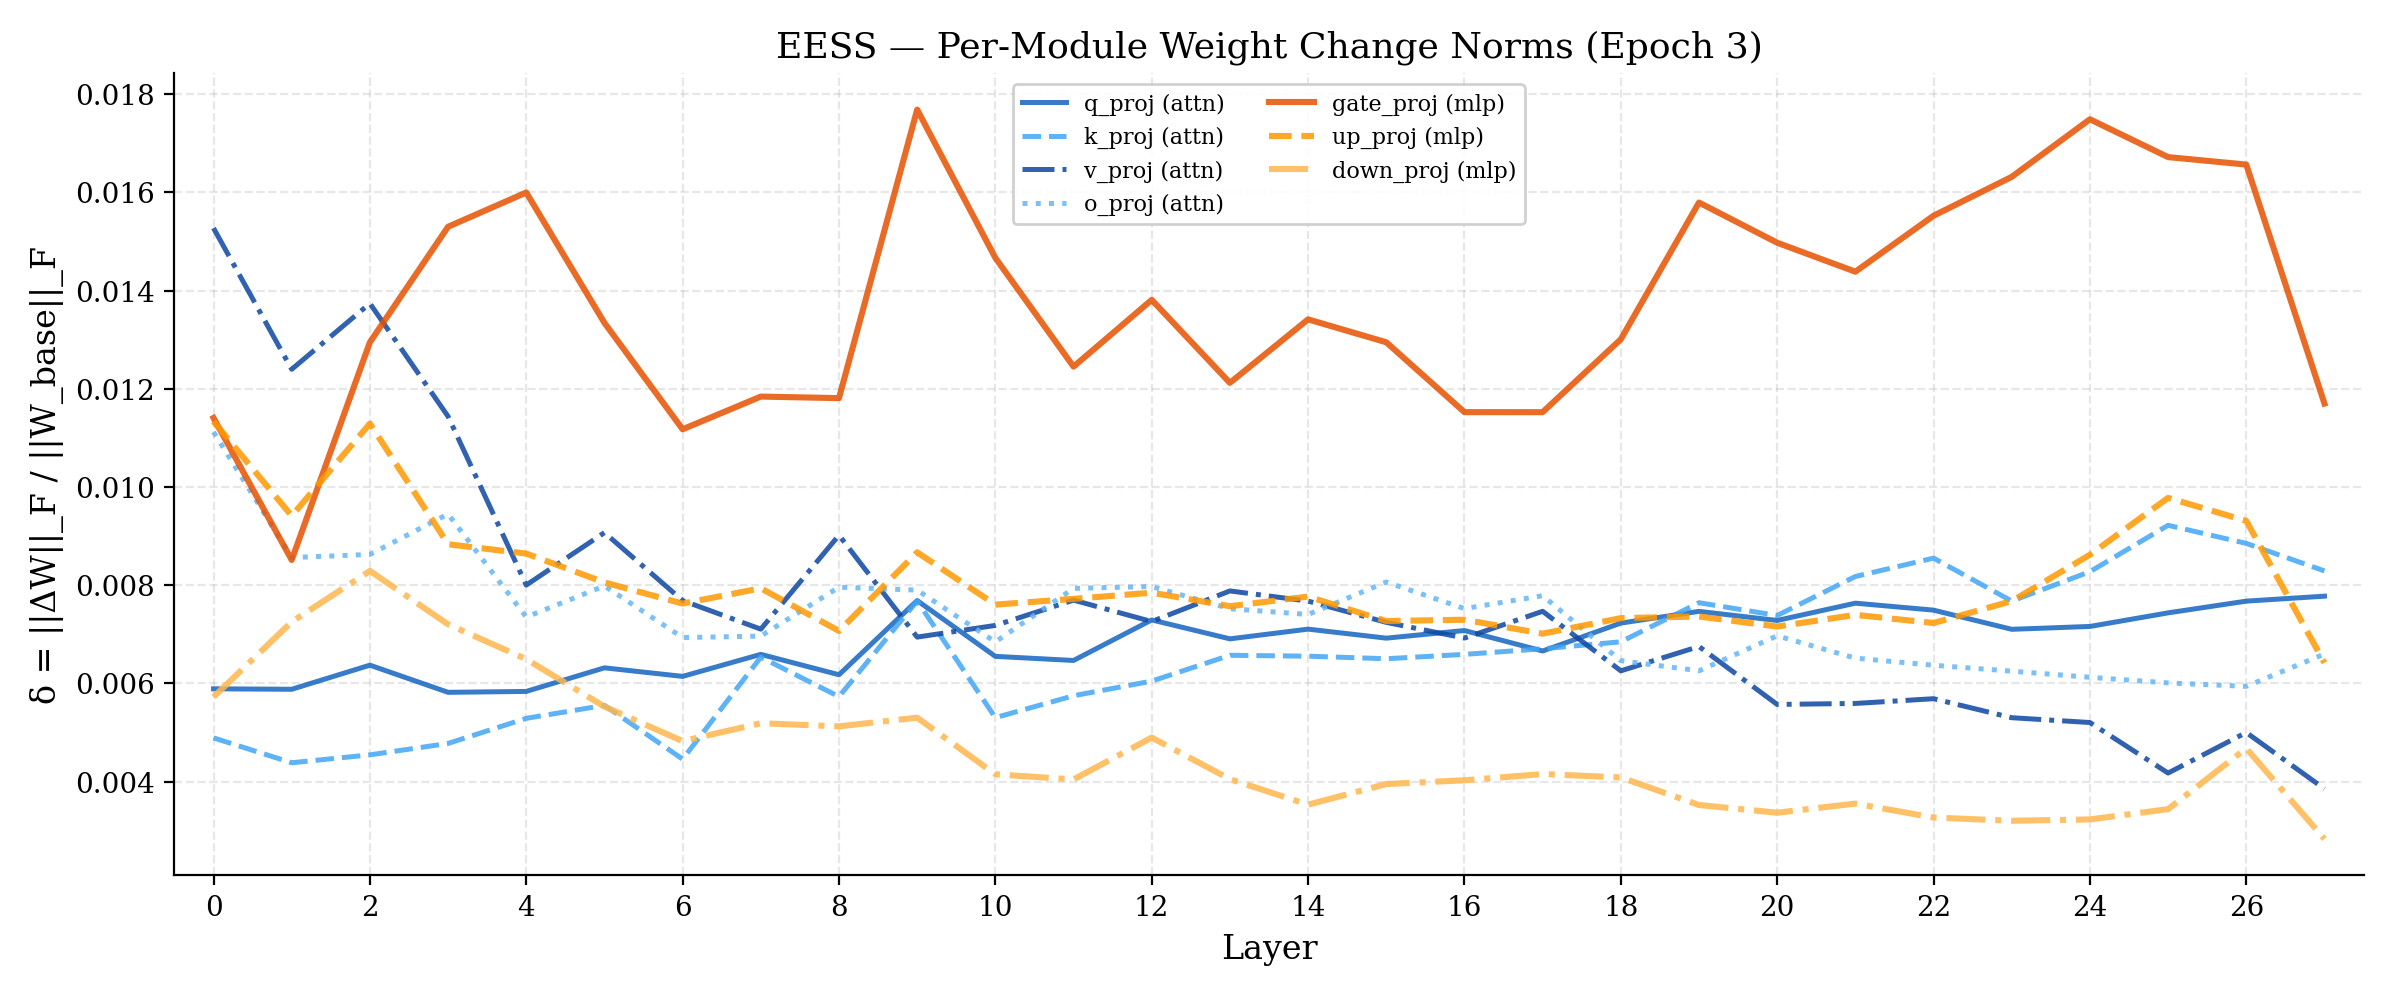
\includegraphics[width=\textwidth]{figures/wcn_eess_detailed.png}
    \caption{Per-module weight change norms (EESS).}
\end{subfigure}
\hfill
\begin{subfigure}[b]{0.48\textwidth}
    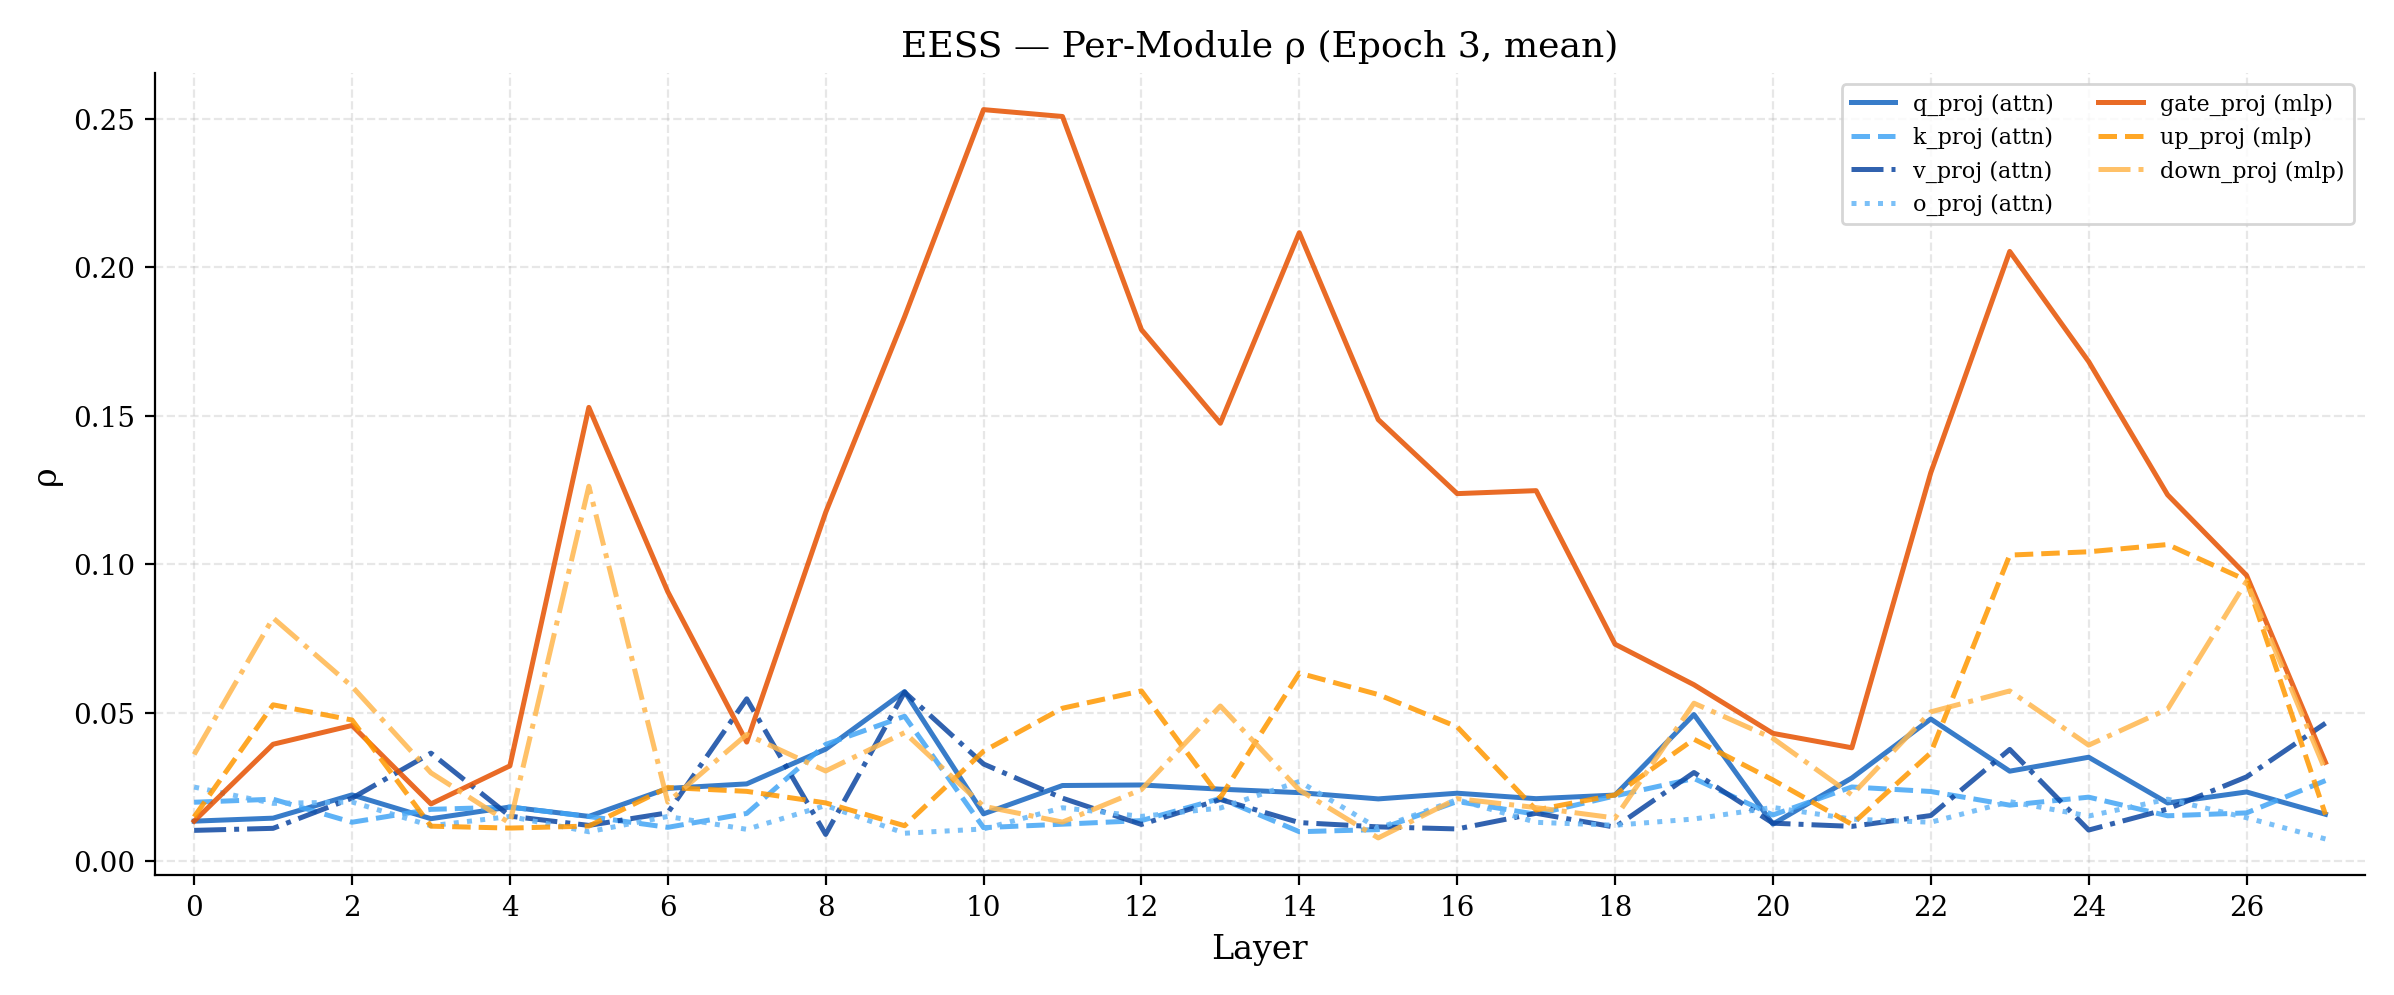
\includegraphics[width=\textwidth]{figures/permod_eess.png}
    \caption{Per-module domain alignment $\rho$ (EESS).}
\end{subfigure}
\caption{The \texttt{gate\_proj} anomaly: in both weight change norms (left) and domain alignment (right), \texttt{gate\_proj} (solid orange) dominates all other modules across layers. The pattern is consistent across domains.}
\label{fig:gate_finding}
\end{figure}

\paragraph{Interpretation.} The gating mechanism provides a natural explanation: \texttt{gate\_proj} selects \emph{which} MLP features are active, making it the first point of domain-specific routing within the MLP block. By modifying $W_{\text{gate}}$, fine-tuning can selectively activate domain-relevant features without changing the actual feature computation ($W_{\text{up}}$) or output projection ($W_{\text{down}}$) as much. This is consistent with the broader attention-router / MLP-executor framework: within the MLP itself, \texttt{gate\_proj} acts as a \emph{sub-router} that directs computation toward domain-specific feature subspaces.


% ======================================================================
\section{Summary}
% ======================================================================

\begin{table}[H]
\centering
\caption{Summary of all three metrics (Epoch 3, averaged across domains).}
\label{tab:summary}
\begin{tabular}{lccc}
\toprule
Metric & Attention & MLP & MLP/Attn \\
\midrule
Weight change norm ($\bar{\delta}$)         & 0.00699 & 0.00920 & 1.31$\times$ \\
Domain mixing MSE (lower = specialised)     & 0.0275  & 0.0118  & 2.33$\times$ \\
Domain alignment $\rho$ (higher = aligned)  & 0.0189  & 0.0559  & 2.96$\times$ \\
\bottomrule
\end{tabular}
\end{table}

All three metrics consistently support the hypothesis: MLP modules adapt \textbf{more} (1.3$\times$ larger updates), \textbf{more specifically} (2.3$\times$ more domain-differentiated), and \textbf{more directionally} (3.0$\times$ more aligned with domain concept vectors) than attention modules. The \texttt{gate\_proj} matrix is the strongest individual contributor, acting as a domain-specific feature amplifier within the SwiGLU architecture.

\end{document}
